\documentclass[a4paper]{article}

\usepackage[french]{babel}
\usepackage[utf8x]{inputenc}
\usepackage{float}
\usepackage[fleqn]{amsmath}
\usepackage{graphicx}
\usepackage[colorinlistoftodos]{todonotes}
\usepackage{ wasysym }
\usepackage{fullpage}

\title{INFO-H-303 - Bases de Données - Projet Villo!}
\author{Florentin Hennecker - Magali Hublet}
\date{2014/2015}

\begin{document}
\maketitle
\tableofcontents

\section{Introduction}

Pour ce projet de bases de données, il nous a été demandé de développer un système de gestion des Villos pour la ville de Bruxelles, avec une interface graphique. Tous les Bruxellois doivent pouvoir utiliser ce système pour naviguer dans la ville à l'aide des vélos mis à disposition ou consulter diverses informations à propos de leur compte.


\section{Modèle entité-relation}

\begin{figure}[H]
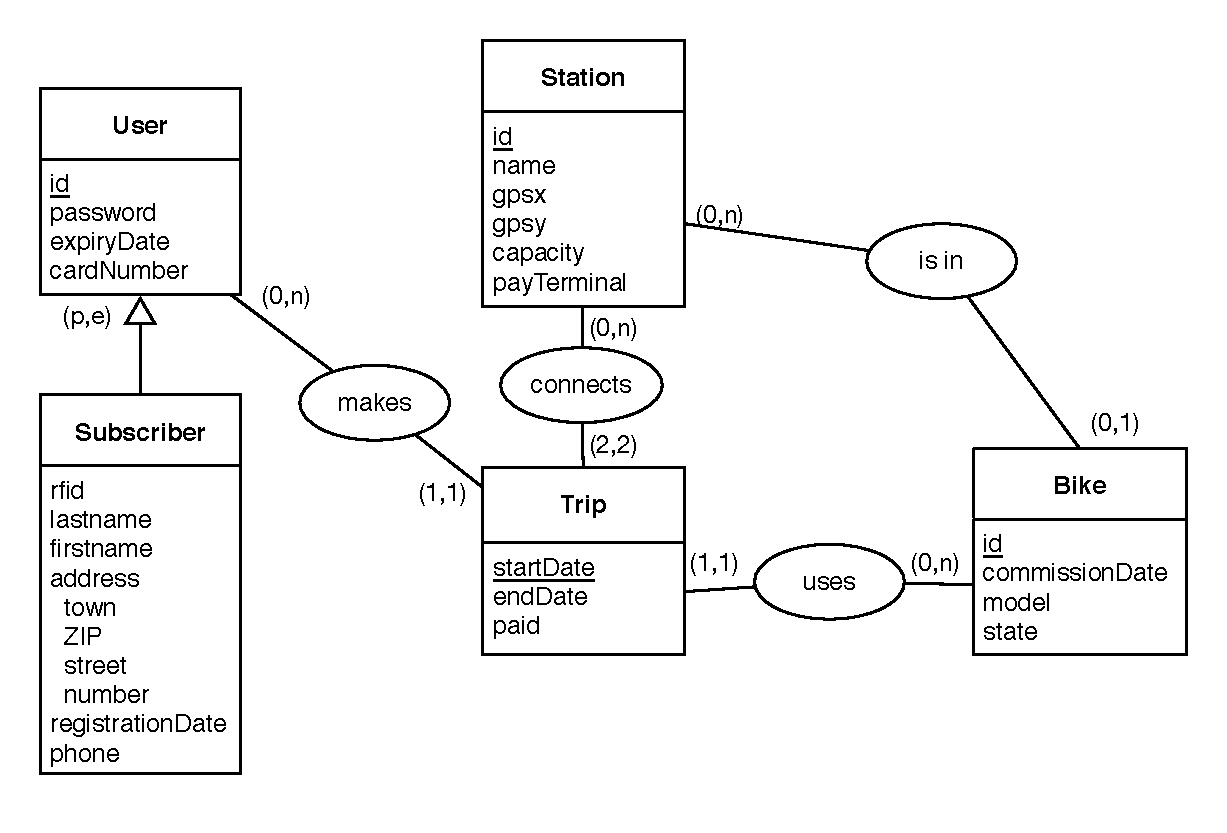
\includegraphics[width=\textwidth]{images/ERSchema.eps}
\end{figure}

Notons que nous avons traduit le modèle rendu lors de la première partie pour mieux coller avec notre code. Nous avons également séparé l'ancien champ \texttt{gps-coord} en deux champs : \texttt{gpsx} et \texttt{gpsy}. La clé d'un Trip est User.id + Trip.startDate.

\subsection{Contraintes d'intégrité}
\begin{itemize}
\item l'heure de départ d'un déplacement est antérieure à l'heure d'arrivée
\item un vélo est impliqué dans maximum un déplacement à un moment donné
\item la date de mise en service d'un vélo est antérieure à toute date de déplacement qui implique ce vélo
\item le nombre de vélos rangés dans une station n'excède pas la capacité de cette station
\item la date d'inscription d'un utilisateur est antérieure à tout déplacement fait par celui-ci
\item la date d'inscription d'un abonné est antérieure à la date d'expiration de son titre de transport
\item la date de départ d'un déplacement est antérieure à la date d'expiration du titre de transport de l'utilisateur qui fait ce déplacement
\item le RFID est unique pour chaque abonné
\item la capacité d'une station est positive
\item un vélo dont l'état spécifie qu'il ne fonctionne pas ne peut pas être utilisé dans un déplacement
\item il ne peut exister plus de deux déplacements non payés impliquant le même utilisateur
\end{itemize}

\subsection{Remarques et hypothèses}
\begin{itemize}
\item Un déplacement implique 2 stations, mais ces stations ne sont pas forcément différentes (un utilisateur peut faire une boucle)
\item Les tickets de 7 jours et de 24 heures sont valables à partir de la date du premier déplacement
\item Les abonnements annuels sont valables à partir du paiement
\end{itemize}

\section{Modèle relationnel}
\begin{itemize}
\item Station(\underline{id}, name, payTerminal, capacity, gpsx, gpsy)
\item Bike(\underline{id}, commissionDate, model, state, station)
    \begin{itemize}
    \item Bike.station référence Station.id
    \end{itemize}
\item User(\underline{id}, password, expiryDate, cardNumber)
\item Subscriber(\underline{id}, RFID, lastName, firstName, addressTown,\\ addressZIP, addressStreet, addressNumber, registrationDate, phone)
    \begin{itemize}
    \item Subscriber.id référence User.id
    \end{itemize}
\item Trip(\underline{user, startDate}, endDate, startstation, endStation, bike, paid) 
    \begin{itemize}
    \item Trip.startStation et Trip.endStation référencent Station.id
    \item Trip.bike référence Bike.id
    \end{itemize}
\end{itemize}

\subsection{Contraintes supplémentaires}
\begin{itemize}
\item Bike.station est unique dans la relation Bike
\item Subscriber.id référence User.id de manière unique
\item Trip.startStation, Trip.endStation et Trip.bike sont uniques dans la relation Déplacement
\end{itemize}


\section{Script SQL DDL}

\begin{verbatim}
CREATE TABLE Stations(
    id          INTEGER         NOT NULL,
    name        TEXT,
    payTerminal INTEGER,
    capacity    INTEGER,
    gpsx        REAL,
    gpsy        REAL,

    PRIMARY KEY (id)
);

CREATE TABLE Bikes(
    id              INTEGER      NOT NULL,
    commissionDate  TEXT,
    model           TEXT,
    state           TEXT,
    station         INTEGER,

    PRIMARY KEY (id),
    FOREIGN KEY (station) REFERENCES Stations(id)
);

CREATE TABLE Users(
    id              INTEGER     NOT NULL,
    password        INTEGER,
    expiryDate      TEXT,
    cardNumber      INTEGER,

    PRIMARY KEY (id)
);

CREATE TABLE Subscribers(
    id                  INTEGER        NOT NULL,
    rfid                INTEGER        UNIQUE,
    lastName            TEXT,
    firstName           TEXT,
    addressTown         TEXT,
    addressZIP          TEXT,
    addressStreet       TEXT,
    addressNumber       TEXT,
    registrationDate    TEXT,
    phone               INTEGER,

    PRIMARY KEY (id),
    FOREIGN KEY (id) REFERENCES Users(id)
);

CREATE TABLE Trips(
    user            INTEGER     NOT NULL,
    startDate       TEXT,
    endDate         TEXT,
    startStation    INTEGER,
    endStation      INTEGER,
    bike            INTEGER,
    paid            INTEGER,

    PRIMARY KEY (user, startDate),
    FOREIGN KEY (user) REFERENCES Users(id),
    FOREIGN KEY (startStation) REFERENCES Stations(id),
    FOREIGN KEY (endStation) REFERENCES Stations(id),
    FOREIGN KEY (bike) REFERENCES Bikes(id)
);
\end{verbatim}

  \subsection{Notes sur le script SQL DDL}

  \paragraph{Types de données} SQLite3 ne supporte pas beaucoup de types de données différents. Il faut donc les choisir en fonction de l'affinité du type de données à stocker pour un des types de base : \texttt{INTEGER, REAL, TEXT} ou \texttt{BLOB}\footnote{https://www.sqlite.org/datatype3.html}.
  
  \paragraph{Typage de Bikes.state} Nous avons choisi d'utiliser un champ de type \texttt{TEXT} qui sera \texttt{NULL} si le vélo fonctionne; et qui contiendra le problème signalé s'il y en a un.

\section{Différentes requêtes}



\subsection{Première requête}
    Les utilisateurs habitant Ixelles ayant utilisé un Villo de la station Flagey.

    \paragraph{SQL}
  \begin{verbatim}
  SELECT DISTINCT Subscribers.id, Subscribers.firstName, Subscribers.lastName
  FROM Trips
  INNER JOIN Subscribers ON Subscribers.id = Trips.user AND Subscribers.addressZIP = "1050"
  INNER JOIN Stations ON Stations.id = Trips.startStation AND Stations.name = "FLAGEY";
  \end{verbatim}
  
    \paragraph{Algèbre relationnelle}
    $$ Subs \leftarrow rename(Subscribers, (id \rightarrow subid))$$
    $$TripsFromSubsInXL \leftarrow Trips\ \Bowtie_{user=subid\ and\ addressZIP='1050'}\ Subs$$
    $$FullResult \leftarrow TripsFromSubsInXL\ \Bowtie_{startStation=id\ and\  name='FLAGEY'}\ Stations$$
    $$Result \leftarrow \pi_{subid}(FullResult)$$
    
    \paragraph{Calcul relationnel tuples}
    $$ \{sub.id | Subscribers(sub) \land sub.addressZIP='1050' \land \exists t (Trips(t)$$
    $$ \land\ \exists s (Stations(s) \land t.startStation=s.id \land s.name = 'FLAGEY'))  \} $$



\subsection{Deuxième requête}
    Les utilisateurs ayant utilisé Villo au moins 2 fois.

    \paragraph{SQL}
  \begin{verbatim}
  SELECT Trips.user, COUNT(*)
  FROM Trips
  GROUP BY Trips.user
  HAVING COUNT(*) >= 2
  ORDER BY Trips.user;
  \end{verbatim}
  
  \paragraph{Algèbre relationnelle}
  $$ TA \leftarrow rename(Trips, (user \rightarrow ua, startDate \rightarrow sa)) $$
  $$ TB \leftarrow rename(Trips, (user \rightarrow ub, startDate \rightarrow sb)) $$
  $$FullResult \leftarrow TA\ \Bowtie_{ua=ba\ and\ sa!=sb}\ TB $$
  $$Result \leftarrow \pi_{ua}(FullResult)$$
  
  \paragraph{Calcul relationnel tuples}
  $$ \{ t_1.user | Trips(t_1) \land \exists t_2 (Trips(t_2) \land t_1.user = t_2.user \land t_1.startDate \neq t_2.startDate)\} $$
  


\subsection{Troisième requête}
    Les paires d'utilisateurs ayant fait un trajet identique.

    \paragraph{SQL}
  \begin{verbatim}
  SELECT DISTINCT TA.user, TB.user
  From Trips AS TA
  INNER JOIN Trips AS TB 
      ON TA.user > TB.user 
      AND TA.startStation = TB.startStation 
      AND TA.endStation = TB.endStation;
  \end{verbatim}
    Le \texttt{ON TA.user < TB.user} permet de ne sélectionner qu'une fois une paire. Si on avait utilisé \texttt{ON TA.user != TB.user}, on aurait eu les deux permutations à chaque fois.
    
    \paragraph{Algèbre relationnelle}
    $$ TA \leftarrow rename(Trips, (user \rightarrow ua, startDate \rightarrow sa, endDate \rightarrow ea)) $$
    $$ TB \leftarrow rename(Trips, (user \rightarrow ub, startDate \rightarrow sb, endDate \rightarrow eb)) $$
    $$ FullResult \leftarrow TA\ \Bowtie_{ua>ub\ and\ sa=sb\ and\ ea=eb}\ TB$$
    $$ Result \leftarrow \pi_{ua, ub} (FullResult) $$

    \paragraph{Calcul relationnel tuples}
    $$ \{ s_1.id, s_2.id | Subscribers(s_1) \land Subscribers(s_2) \land s_1.id \neq s_2.id $$
    $$ \land\ \exists t_1, t_2 (Trips(t_1) \land Trips(t_2) \land t_1.user = s_1.id \land t_2.user = s_2.id $$
    $$ \land\ t_1.startStation = t_2.startStation \land t_1.endStation = t_2.endStation) \} $$



\subsection{Quatrième requête}
    Les vélos ayant deux trajets consécutifs disjoints (station de retour du premier trajet différente de la station de départ du suivant)

    \paragraph{SQL}
  \begin{verbatim}
  SELECT DISTINCT TA.bike
  FROM Trips AS TA
  INNER JOIN Trips AS TB
      ON TA.bike = TB.bike
      AND TA.endDate < TB.startDate
  GROUP BY TB.startDate
  HAVING TA.endStation != TB.startStation;
  \end{verbatim}
  
    \paragraph{Algèbre relationnelle}
    $$ TA \leftarrow rename(Trips, (startDate \rightarrow sda, endStation \rightarrow esa, bike \rightarrow ba)) $$
    $$ TB \leftarrow rename(Trips, (startDate \rightarrow sdb, startStation \rightarrow ssb)) $$
    $$ Joint \leftarrow TA\ \Bowtie_{sda < sdb}\ TB $$
    $$ Consec \leftarrow \gamma_{sda}(Joint) $$
    $$ Disjoint \leftarrow \sigma_{esa \neq ssb}(Consec)$$
    $$ Result \leftarrow \pi_{ba}(Disjoint)$$
    
    \paragraph{Calcul relationnel tuples}
    $$ \{ b_1.id | Bikes(b_1) \land \exists t_1, t_2 (Trips(t_1) \land Trips(t_2) \land $$
    $$ \land t_1.startDate < t_2.startDate \land \forall t_3 Trips(t_3) \rightarrow (\lnot (t_3.startDate \geq t_1.startdate \land t_3.startDate \leq t_2.startDate)$$
    $$ \land t_1.endStation \neq t_2.startStation)\}$$

\subsection{Cinquième requête}
    Les utilisateurs, la date d'inscription, le nombre total de trajets effectués, la distance totale parcourue et la distance moyenne parcourue par trajet, classés en fonction de la distance totale parcourue.
    
    \textbf{Remarque :} SQLite3, le système de bases de données que nous avons choisi ne supporte que très peu de fonctions mathématiques. Il a donc fallu écrire une extension C (voir annexe \ref{extension-c}) pour calculer la distance entre deux points données par des coordonnées géographiques. Il suffit ensuite de la compiler en librairie dynamique et de la charger au run-time (\texttt{.load ../distance}).
    
    \textbf{Remarque bis :} La requête demande de classer les utilisateurs mais de sélectionner également la date d'inscription qui n'est donnée que pour les abonnés (y compris dans les données de départ). On effectue donc la requête uniquement pour les abonnés.

    \paragraph{SQL}
  \begin{verbatim}
  .load ../distance
  SELECT  Trips.user, 
          Subscribers.registrationDate, 
          COUNT(*), 
          SUM(distance(SA.gpsx, SA.gpsy, SB.gpsx, SB.gpsy)) AS sum,
          AVG(distance(SA.gpsx, SA.gpsy, SB.gpsx, SB.gpsy)) AS avg
  FROM Trips
  INNER JOIN Subscribers
      ON Trips.user = Subscribers.id
  INNER JOIN Stations AS SA
      ON Trips.startStation = SA.id
  INNER JOIN Stations AS SB
      ON Trips.endStation = SB.id
  GROUP BY Trips.user
  ORDER BY sum DESC;
  \end{verbatim}
  
  \paragraph{Sortie de la requête SQL} Au cas où surviendraient des problèmes avec l'extension C, voici les quelques premières lignes des résultats de l'exécution de la reqûete (la distance est en kilomètres):
    
    \begin{verbatim}
1|2010-01-02T02:44:33|370|1207.94934396373|3.26472795665873
0|2010-01-01T10:00:00|409|1190.54228771068|2.91086133914591
2|2010-01-02T12:15:48|354|1124.53287926094|3.17664655158457
3|2010-01-03T05:53:59|354|1084.18212976889|3.06266138352793
5|2010-01-04T06:27:54|325|1005.28951449224|3.09319850612996
4|2010-01-03T17:51:02|305|980.915784946898|3.21611732769475
6|2010-01-04T20:29:00|303|922.234209777715|3.04367725999246
7|2010-01-05T16:13:48|296|911.168348069189|3.07827144617969
8|2010-01-06T11:14:30|283|890.876347993064|3.14797296110623
12|2010-01-08T13:46:05|282|890.682568600884|3.15844882482583
10|2010-01-07T11:59:56|291|890.305205610363|3.05946806051671
17|2010-01-11T13:28:50|253|837.420477326081|3.30996236097265
16|2010-01-11T04:33:00|265|832.237773879973|3.14051990143386
19|2010-01-13T00:07:57|264|824.574666502193|3.12338888826588
11|2010-01-08T01:19:31|271|822.930182199801|3.03664273874465
9|2010-01-06T23:52:19|266|818.752562810762|3.07801715342392
18|2010-01-12T10:22:17|250|816.105134849112|3.26442053939645
15|2010-01-10T13:17:47|248|802.891594967705|3.23746610874075
    \end{verbatim}



\subsection{Sixième requête}
    Les stations avec le nombre total de vélos déposés dans cette station (un même vélo peut être comptabilisé plusieurs fois) et le nombre d'utilisateurs différents ayant utilisé la station et ce pour toutes les stations ayant été utilisées au moins 10 fois.

    \paragraph{SQL}
  \begin{verbatim}
  SELECT stationA, bikecount, usercount FROM 
      (SELECT endStation AS stationA, COUNT(*) AS bikecount
      FROM Trips AS TA
      GROUP BY endStation
      HAVING COUNT(*) >= 10)
  INNER JOIN
      (SELECT endStation AS stationB, COUNT(DISTINCT user) AS usercount
      FROM Trips AS TB
      GROUP BY endStation)
  ON stationA = stationB;
  \end{verbatim}




\section{Application}

    \subsection{Technologies utilisées et architecture}
    Nous avons utilisé Flask\footnote{http://flask.pocoo.org/docs/0.10/}, un serveur web, générateur de pages dynamiques en Python; couplé avec SQLite3. Python est un langage très rapide en termes de temps de développement et nous a donc permis de prototyper l'application en quelques lignes.\\
    
    Le choix de SQLite3 s'est avéré agréable au début puisque toute l'application (BDD comprise) était contenue dans un seul dossier; il était facile de créer et d'accéder à la base de données. Ce choix a présenté un inconvénient lorsqu'il fallut implémenter la requête 5 demandant de calculer une distance. N'ayant à notre disposition ni de racine carrée, ni de fonction trigonométrique, il a fallu chercher une solution un peu exotique (voir annexe \ref{extension-c}).\\
    
    Flask gère donc les requêtes HTTP envoyées par les clients (fichier \texttt{main.py}), répond en interrogeant la base de données (toutes les requêtes se situent dans le fichier \texttt{requests.py}) et en générant une page html à partir de templates \texttt{jinja2} (dossier \texttt{templates/}).
    
    \subsection{Initialisation}
    Le \texttt{README.md} est voulu assez complet quant à l'installation des dépendances nécessaires et l'initialisation des données. Voici cependant un petit rappel des commandes à effectuer dans le dossier \texttt{src/}:
    
    \begin{verbatim}
    python buildModel.py    # création de la base de données
    python importData.py    # importation des données
    ./lrebuild.sh           # reconstruction des fichiers de langage
    ./lcompile.sh           # compilation des traductions
    python main.py          # lancement du programme
    \end{verbatim}
    
    \subsection{Fonctionnement}
    Toutes les fonctionnalités demandées dans l'énoncé ont été implémentées; elles ont été accompagnées de différents ajouts facultatifs. La gestion des paiements a bien évidemment été simulée. Certaines fonctionnalités ne seront pas présentées ici, comme la génération aléatoire des RFID pour un souci de clarté.
    
    \subsubsection{Utilisateur non connecté}
    Un utilisateur connecté peut faire plusieurs choses, la première étant d'accéder à la page d'accueil (fig \ref{fig-s1}). Il peut également consulter la liste des stations (fig \ref{fig-s2}) sans toutefois avoir la permission de prendre un vélo qui y est déposé (voir boutons grisés en fig \ref{fig-s3}).
    \begin{figure}
    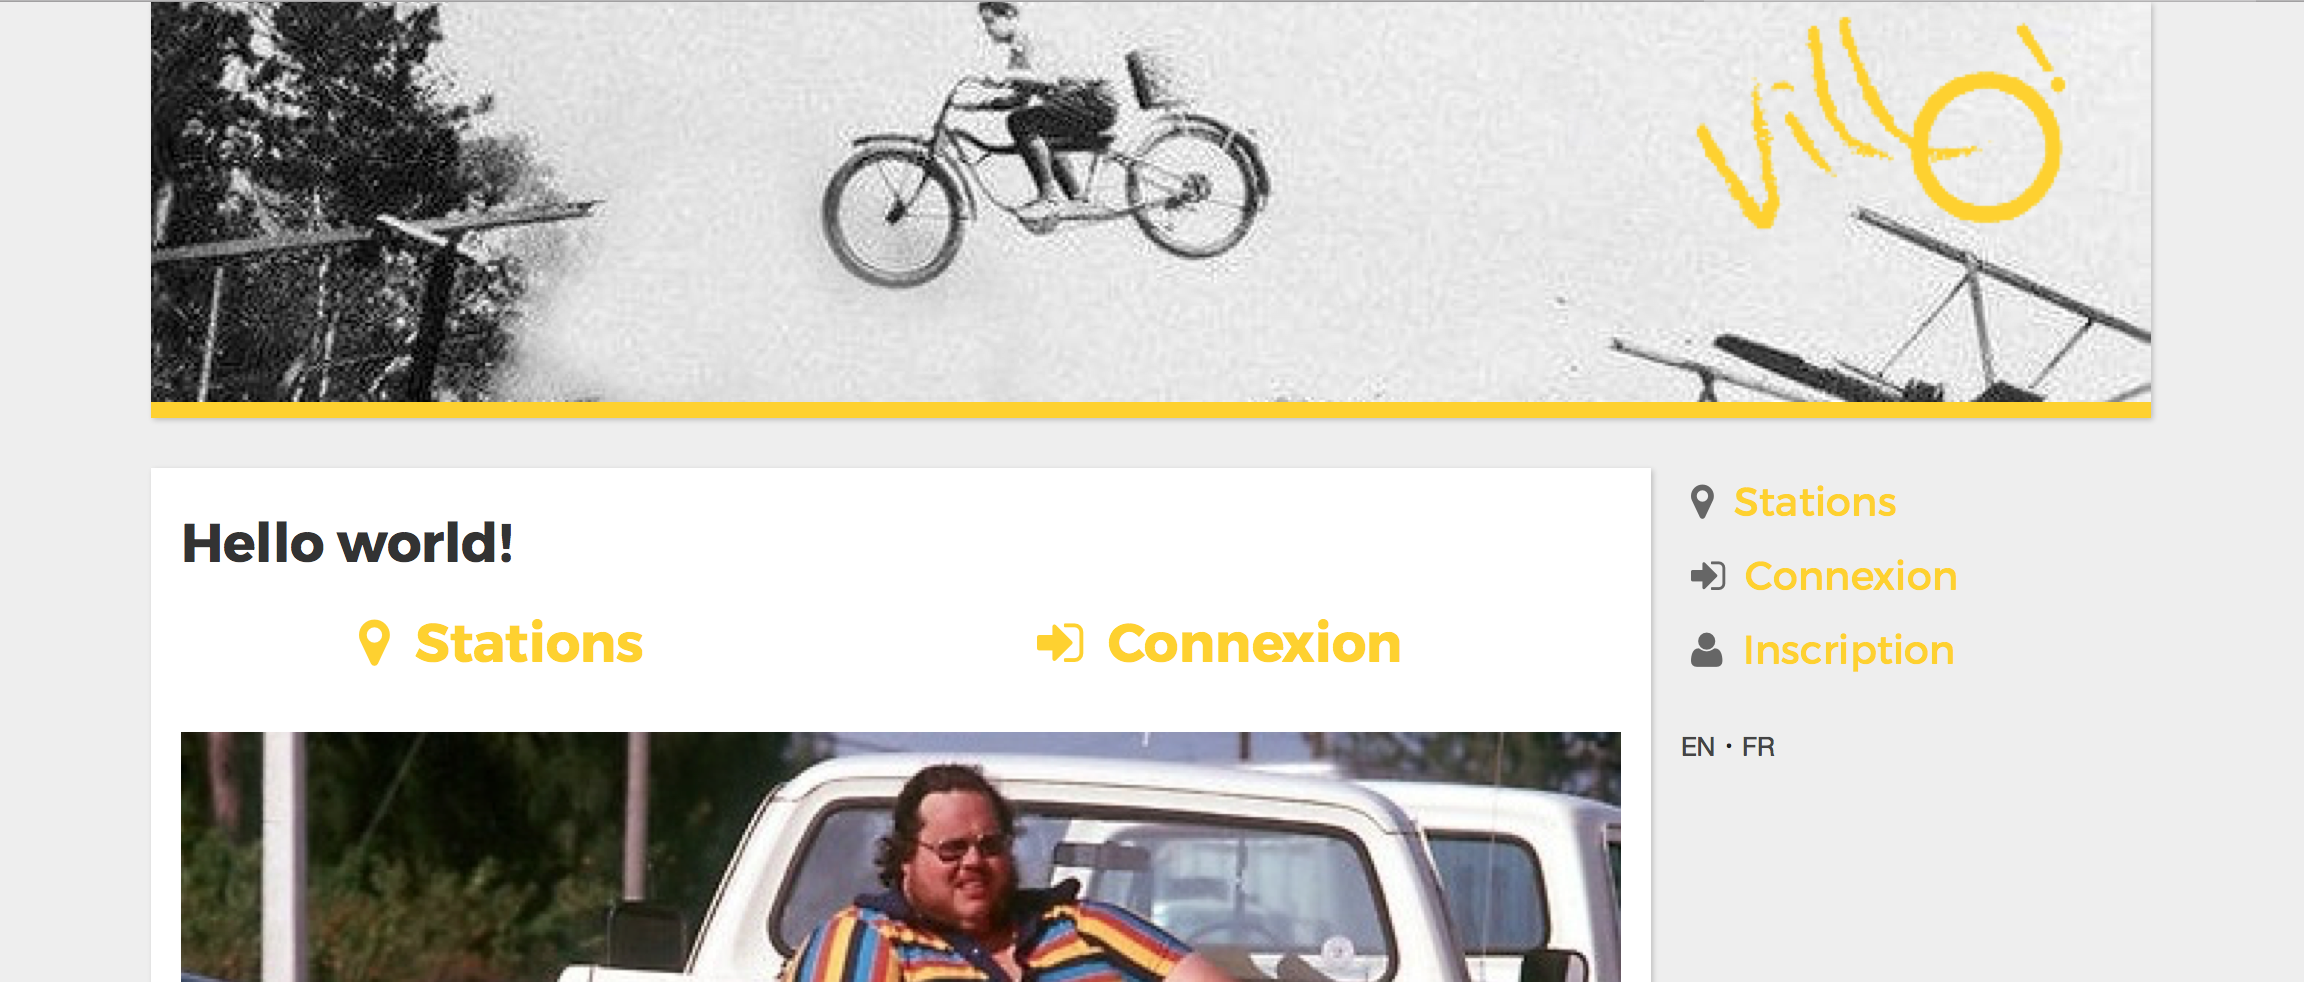
\includegraphics[width=\textwidth]{images/s1.png}
    \caption{Page d'accueil}
    \label{fig-s1}
    \end{figure}
    
    \begin{figure}
    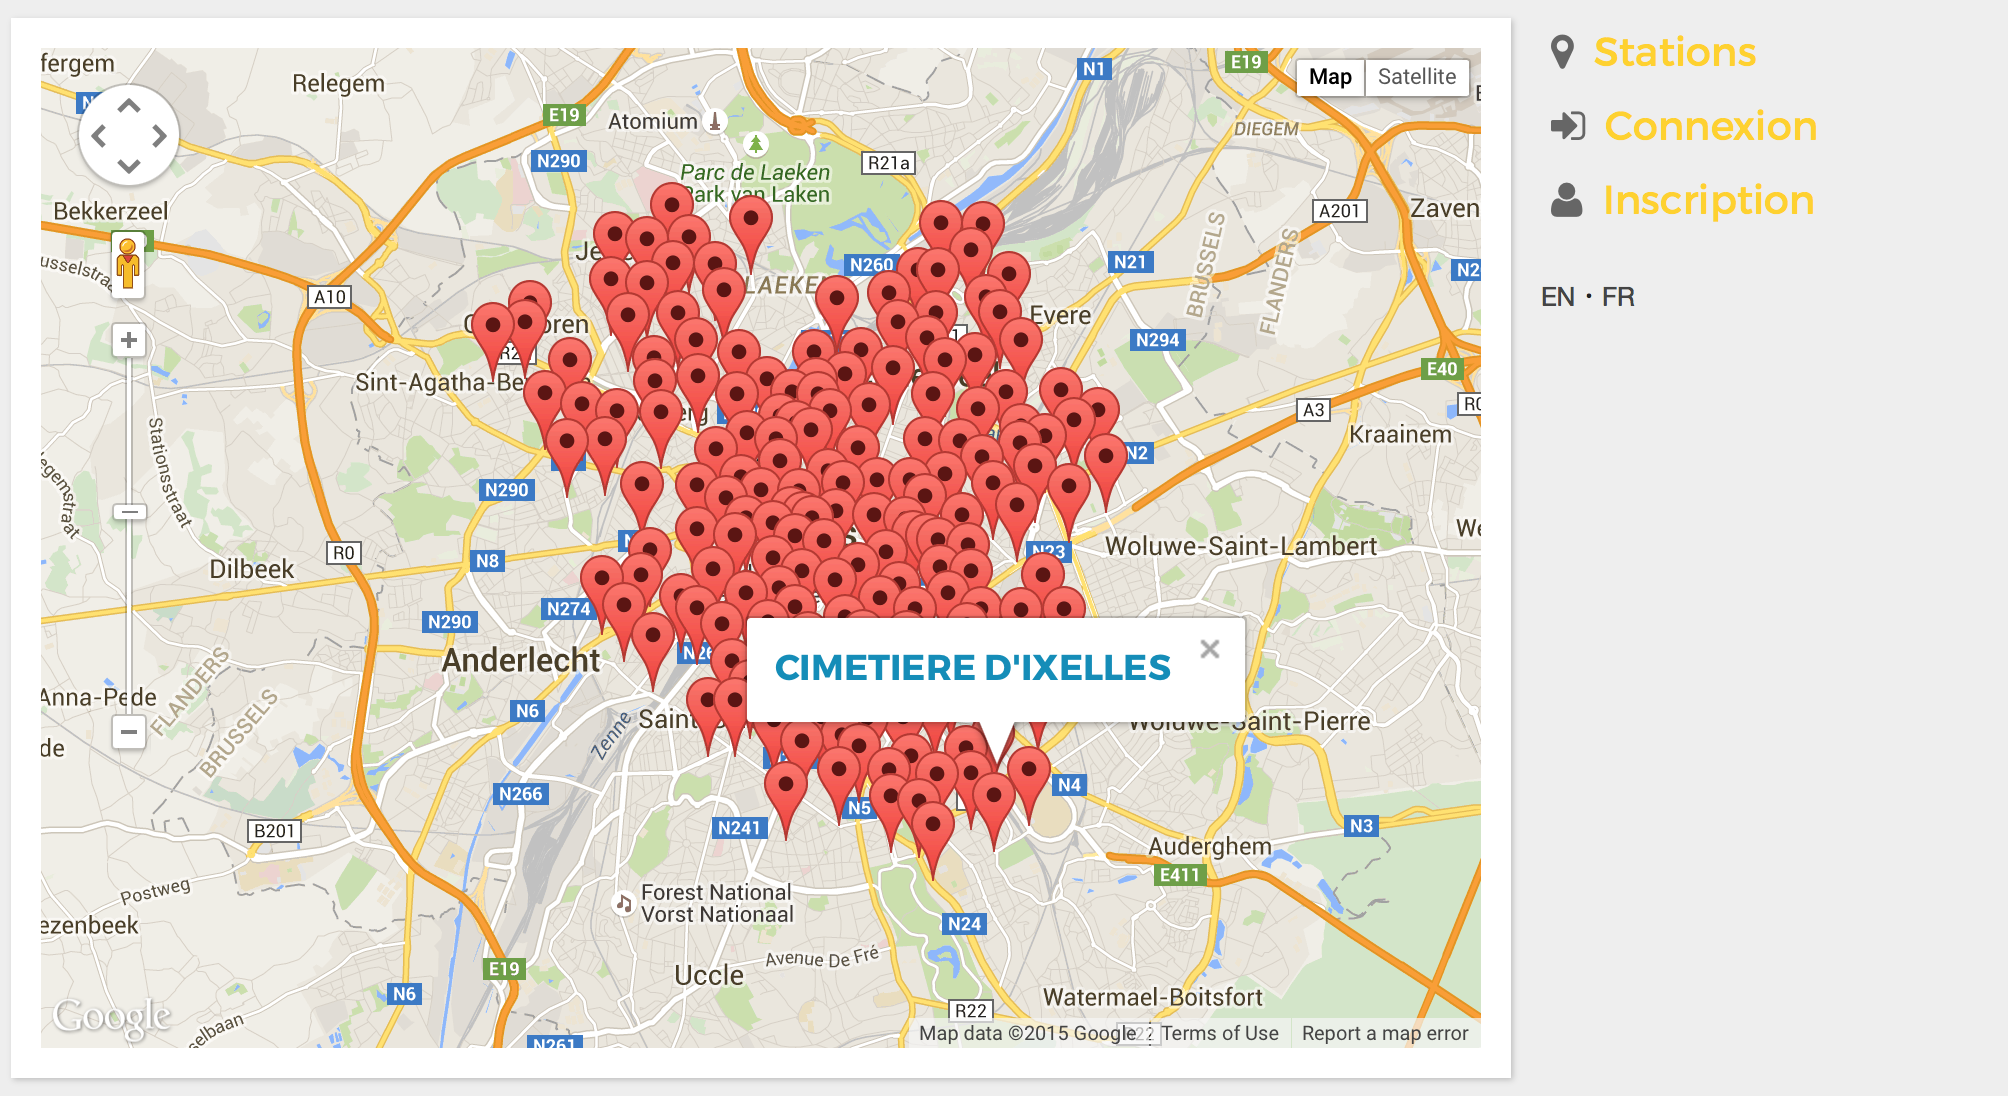
\includegraphics[width=\textwidth]{images/s2.png}
    \caption{Liste des stations}
    \label{fig-s2}
    \end{figure}
    
    \begin{figure}
    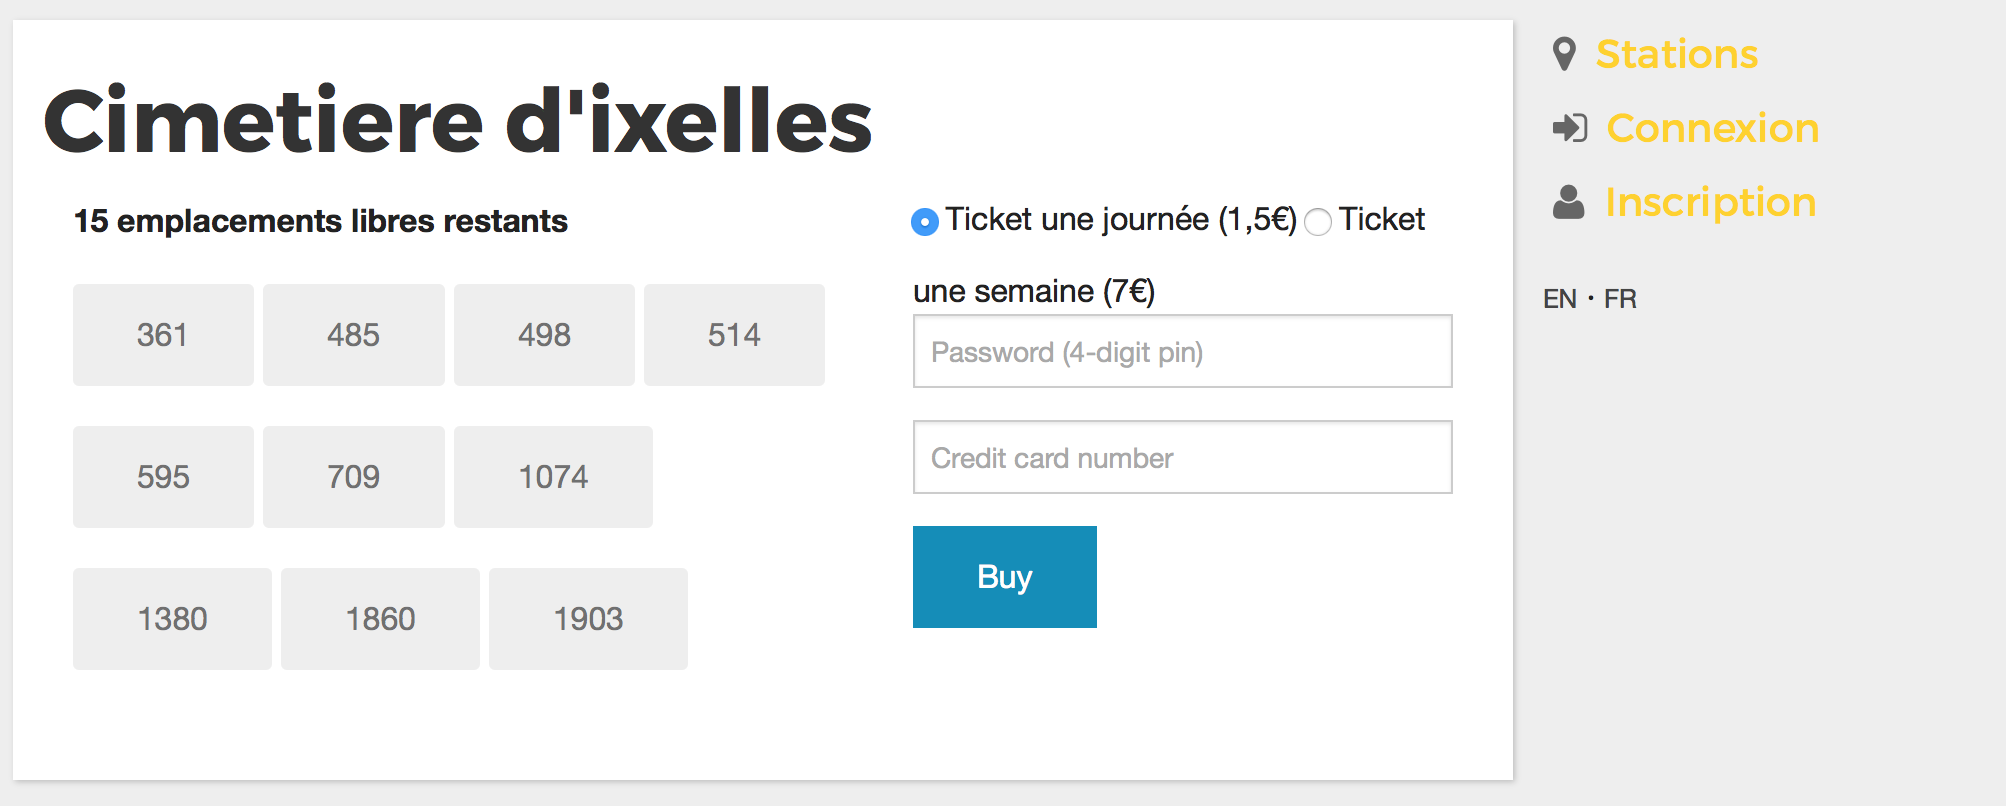
\includegraphics[width=\textwidth]{images/s3.png}
    \caption{Vélos inaccessibles pour un utilisateur non-connecté}
    \label{fig-s3}
    \end{figure}
    
    \subsubsection{Enregistrement d'un nouvel utilisateur}
    Enregistrons-nous comme nouvel abonné. Nous sommes face à un formulaire qui est validé autant du côté client (pour produire les messages d'erreur comme en fig \ref{fig-s4}) que du côté serveur (au cas où un utilisateur malveillant forgerait un POST)\footnote{Tous les formulaires présents dans l'application sont vérifiés autant du côté client que du côté serveur}. Après avoir rempli le formulaire, nous atterrissons sur une page qui nous donne notre \texttt{userid} (fig \ref{fig-s5}). 
    
    \begin{figure}
    \begin{center}
    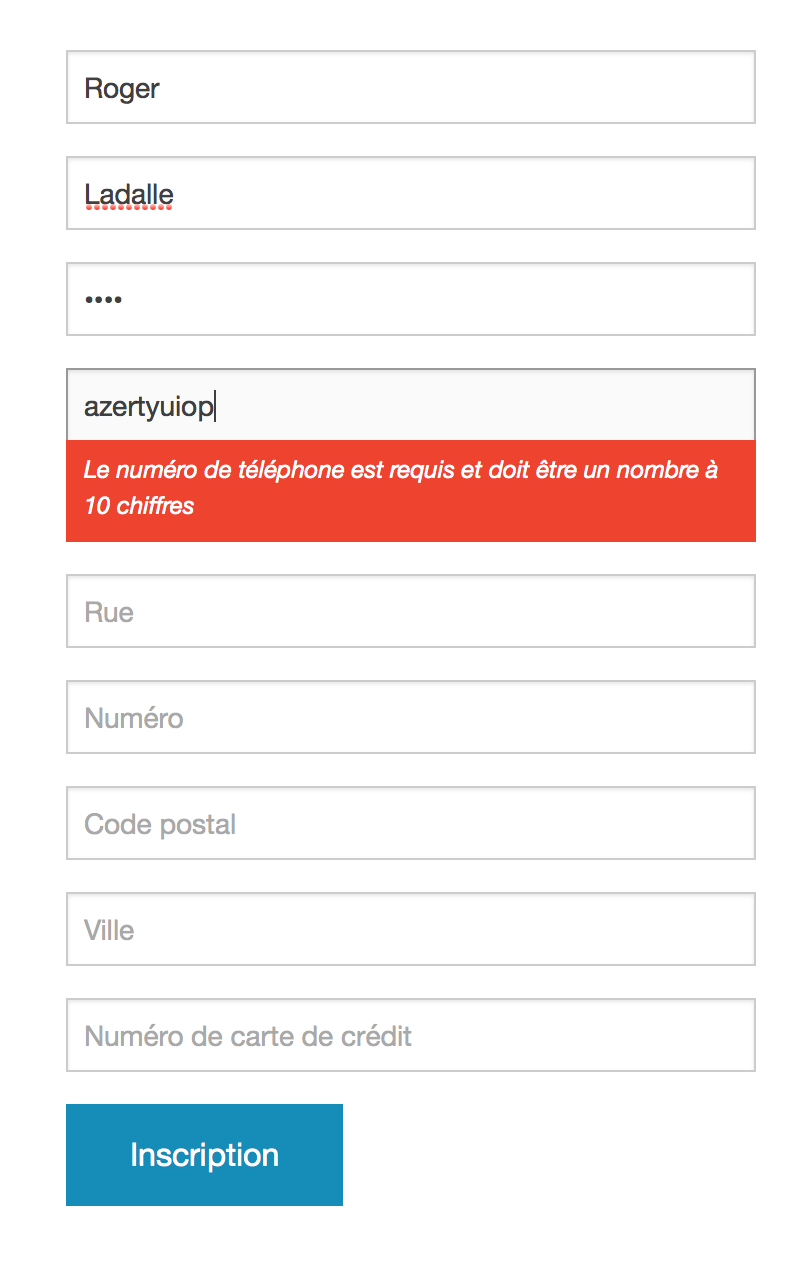
\includegraphics[width=\textwidth/2]{images/s4.png}
    \end{center}
    \caption{Formulaire d'enregistrement}
    \label{fig-s4}
    \end{figure}
    
    \begin{figure}
    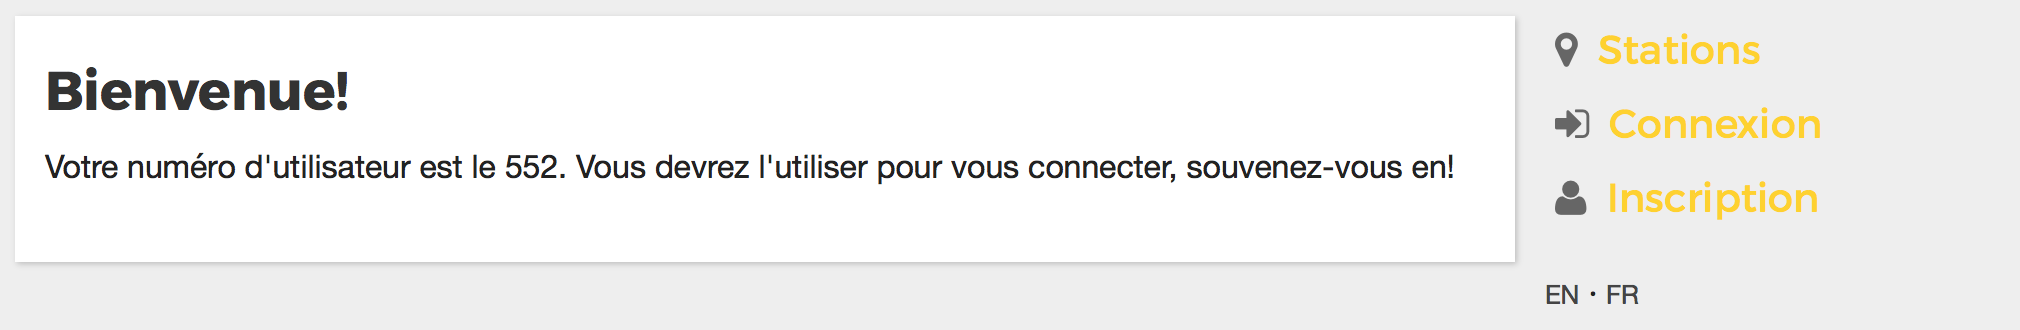
\includegraphics[width=\textwidth]{images/s5.png}
    \caption{Page de bienvenue}
    \label{fig-s5}
    \end{figure}
    
    \subsubsection{Abonné connecté}
    Nous nous connectons (fig \ref{fig-s6}) et nous arrivons sur la page d'accueil qui nous souhaite la bienvenue et qui nous propose plus d'options (fig \ref{fig-s7})!
    
    \begin{figure}
    \begin{center}
    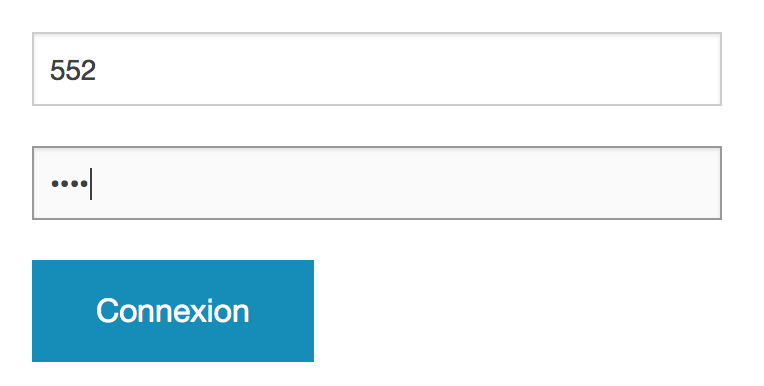
\includegraphics[width=\textwidth/3]{images/s6.png}
    \end{center}
    \caption{Formulaire de connexion}
    \label{fig-s6}
    \end{figure}
    
    \begin{figure}
    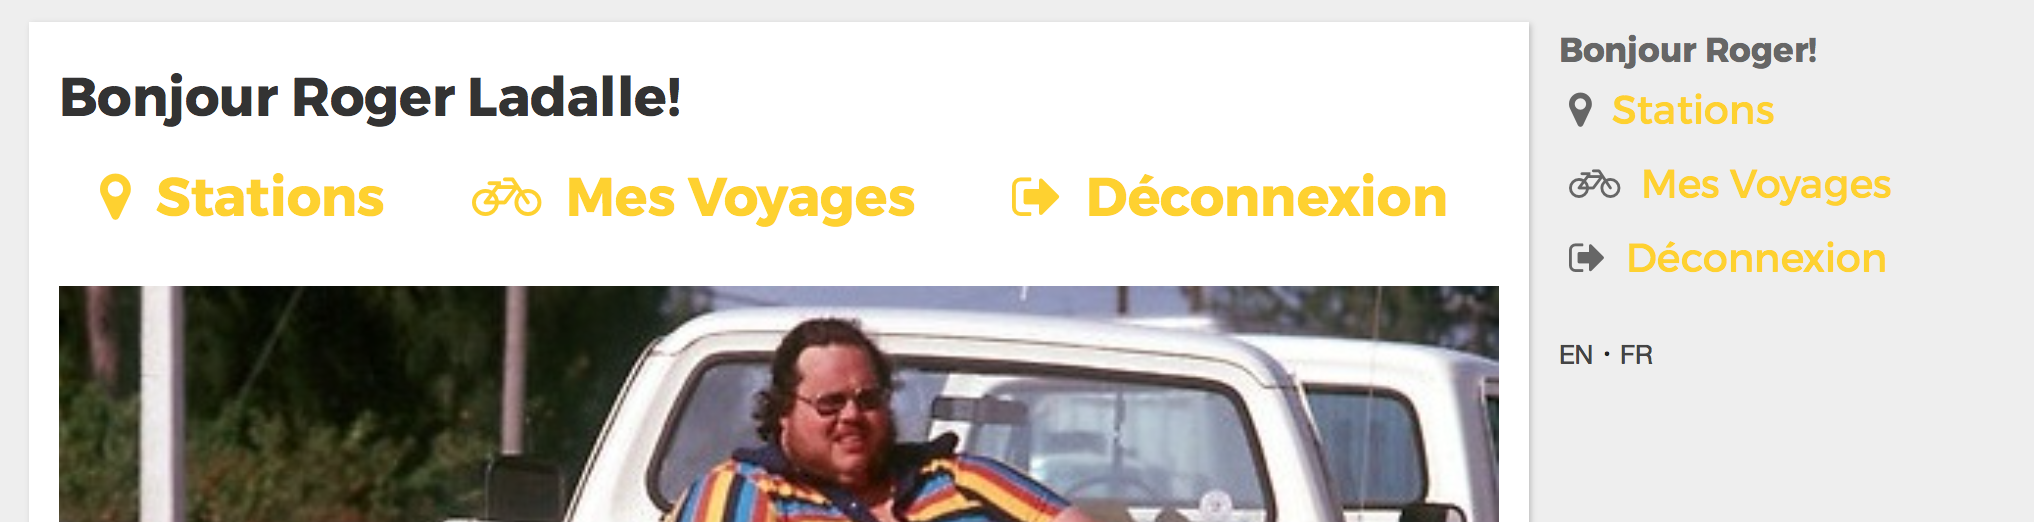
\includegraphics[width=\textwidth]{images/s7.png}
    \caption{Page d'accueil une fois connecté}
    \label{fig-s7}
    \end{figure}
    
    \subsubsection{Effectuer un trajet}
    Prenons le vélo 485 au Cimetière d'Ixelles (fig \ref{fig-s8}). Nous arrivons sur une page qui nous indique les différentes statistiques de notre trajet courant (fig \ref{fig-s9}). Un peu plus tard, nous allons voir la page "Mes trajets" et nous pouvons voir le prix que le trajet nous coûtera (fig \ref{fig-s10}).
    
    \begin{figure}
    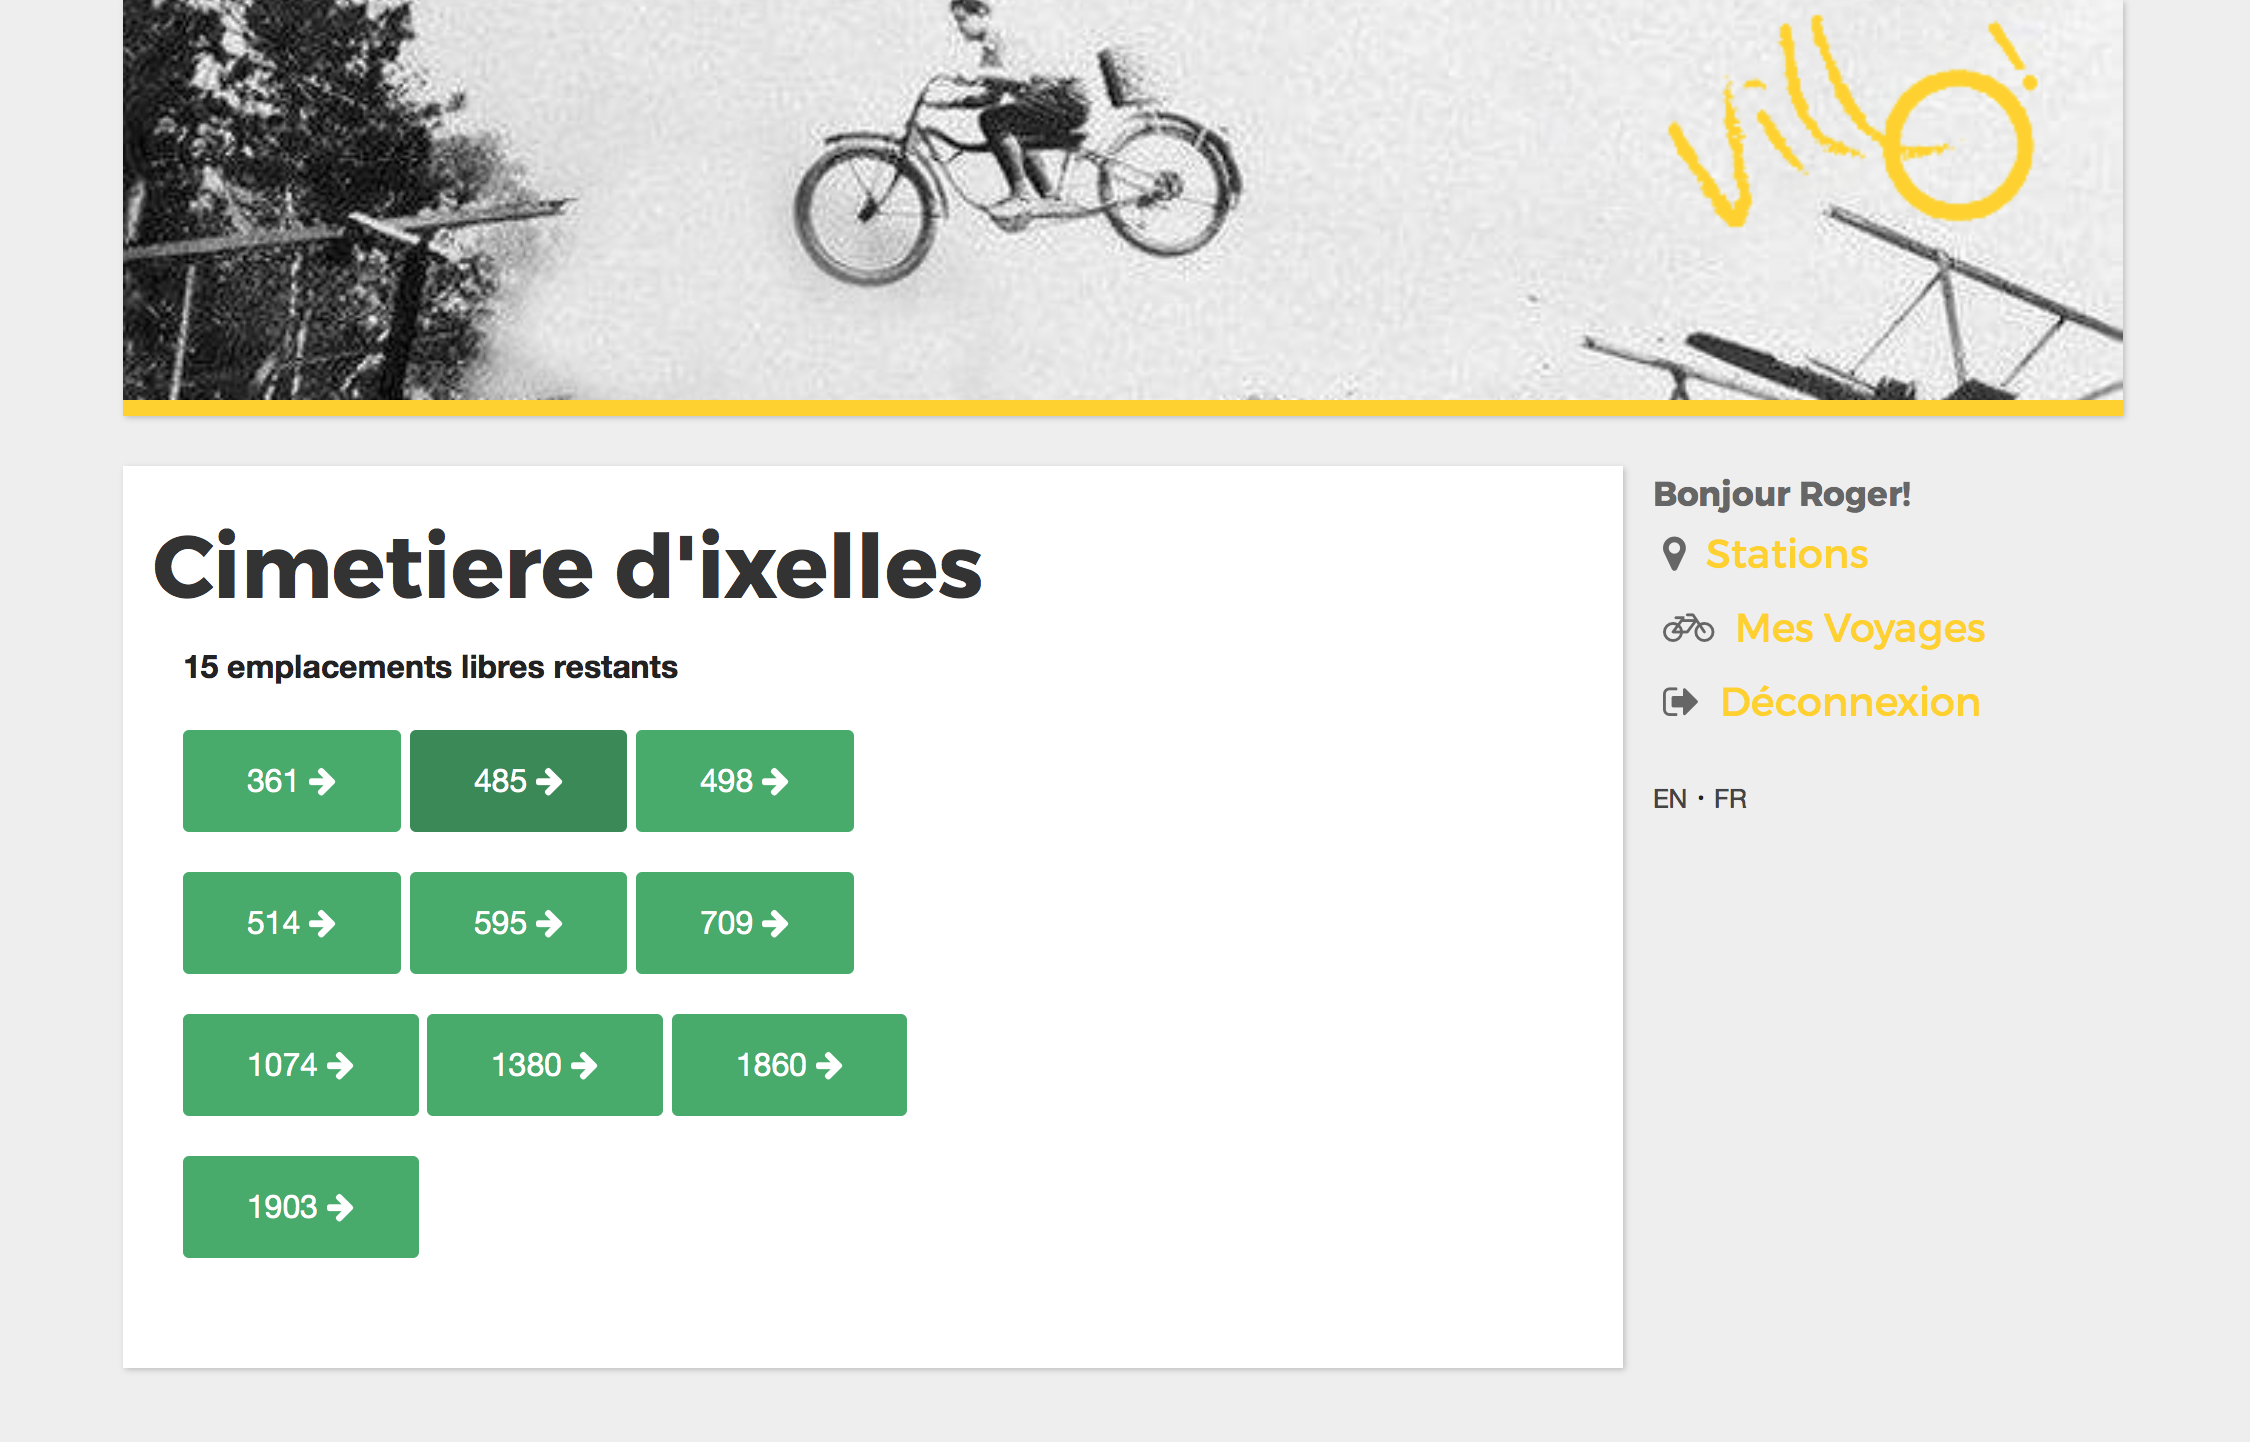
\includegraphics[width=\textwidth]{images/s8.png}
    \caption{Nous prenons le vélo 485}
    \label{fig-s8}
    \end{figure}
    
    \begin{figure}
    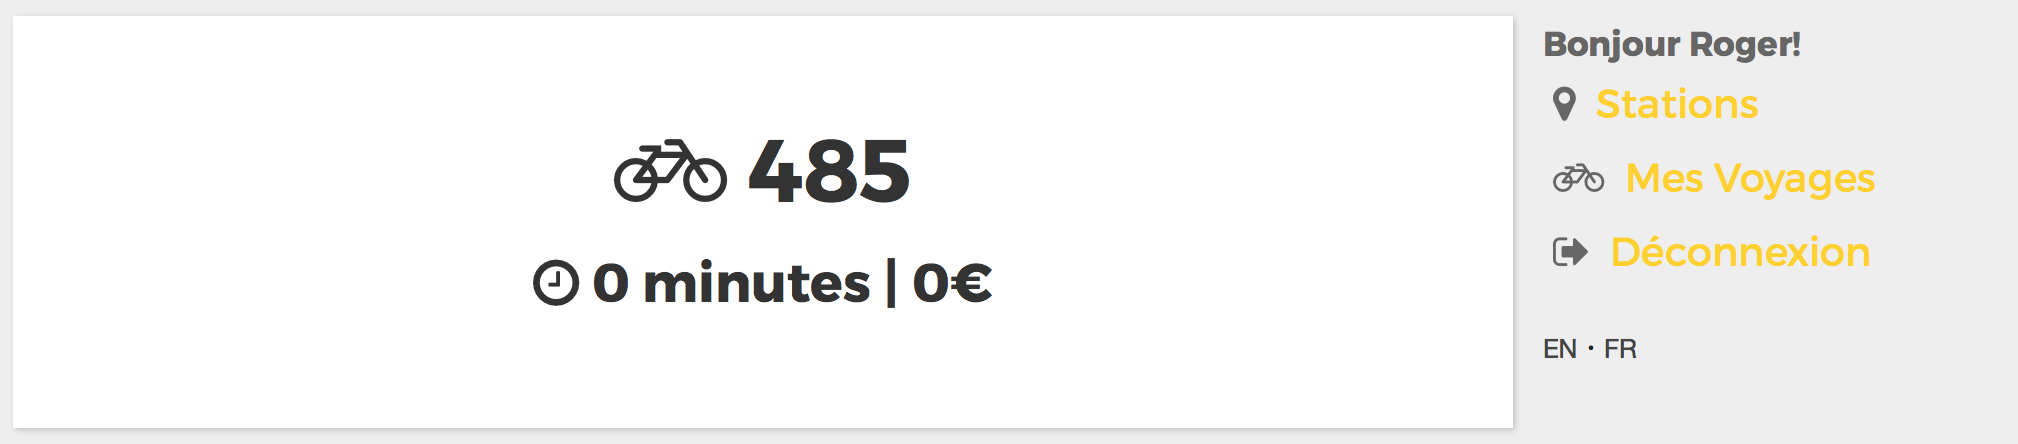
\includegraphics[width=\textwidth]{images/s9.png}
    \caption{Infos du voyage courant}
    \label{fig-s9}
    \end{figure}
    
    \begin{figure}
    \label{fig-s10}
    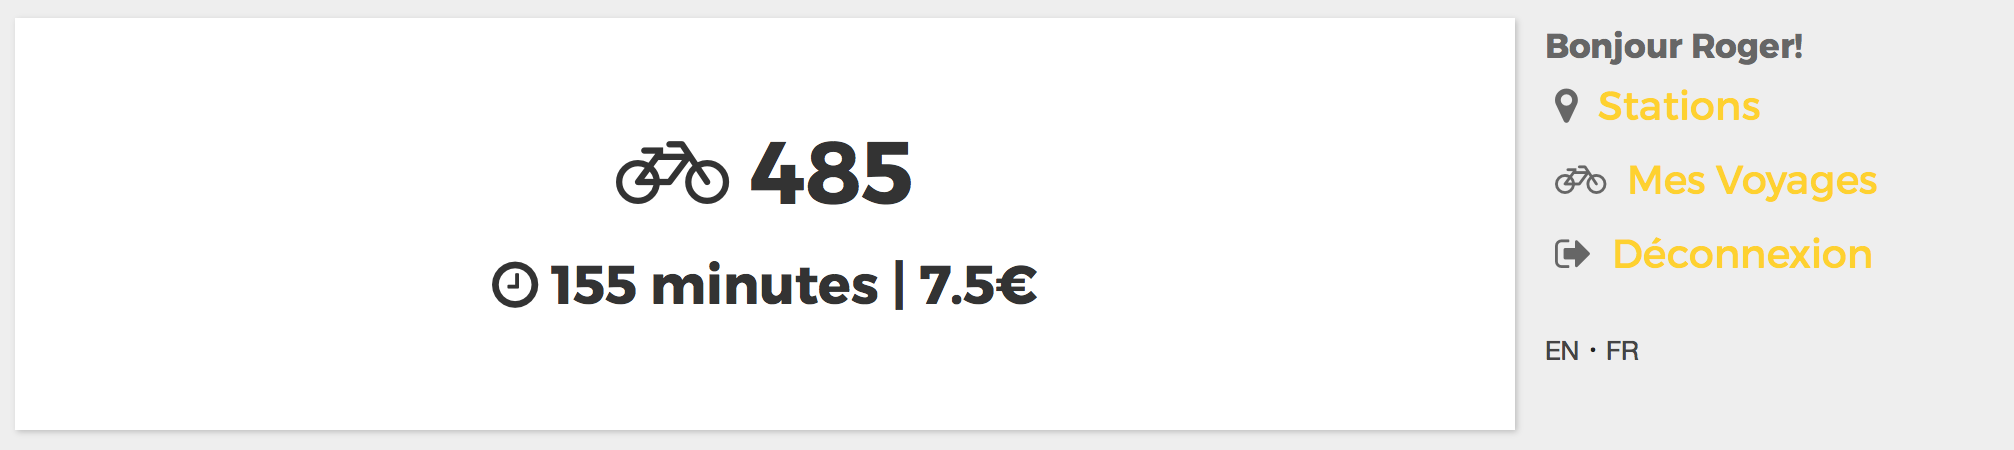
\includegraphics[width=\textwidth]{images/s10.png}
    \caption{Mes voyages}
    \end{figure}
    
    \subsubsection{Signaler un vélo}
    Nous avons terminé notre trajet, nous allons déposer mon vélo à Riga. Seulement, il y a eu quelques problèmes avec la selle et il faut les signaler (fig \ref{fig-s12}). On voit qu'une fois le vélo déposé, il n'est plus accessible (fig \ref{fig-s13}). Voilà, notre premier trajet est effectué (fig \ref{fig-s14})! Encore heureux: quelques minutes après, la station Riga était pleine (fig \ref{fig-s15}).
    
    \begin{figure}
    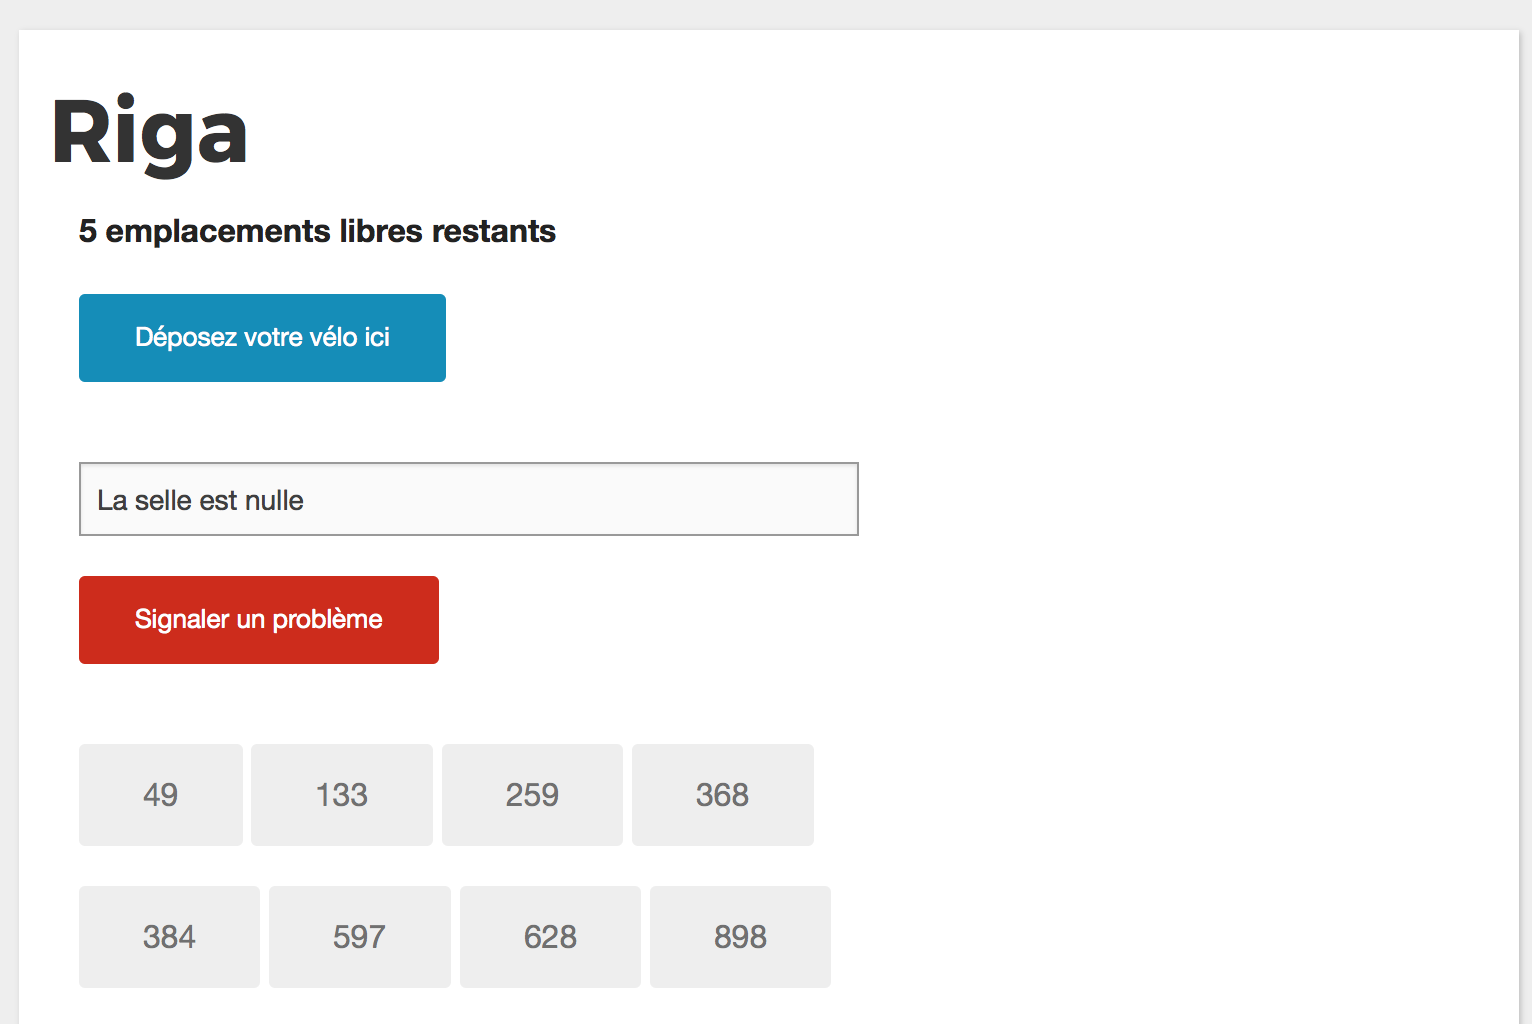
\includegraphics[width=\textwidth]{images/s12.png}
    \caption{Signaler un vélo}
    \label{fig-s12}
    \end{figure}
    
    \begin{figure}
    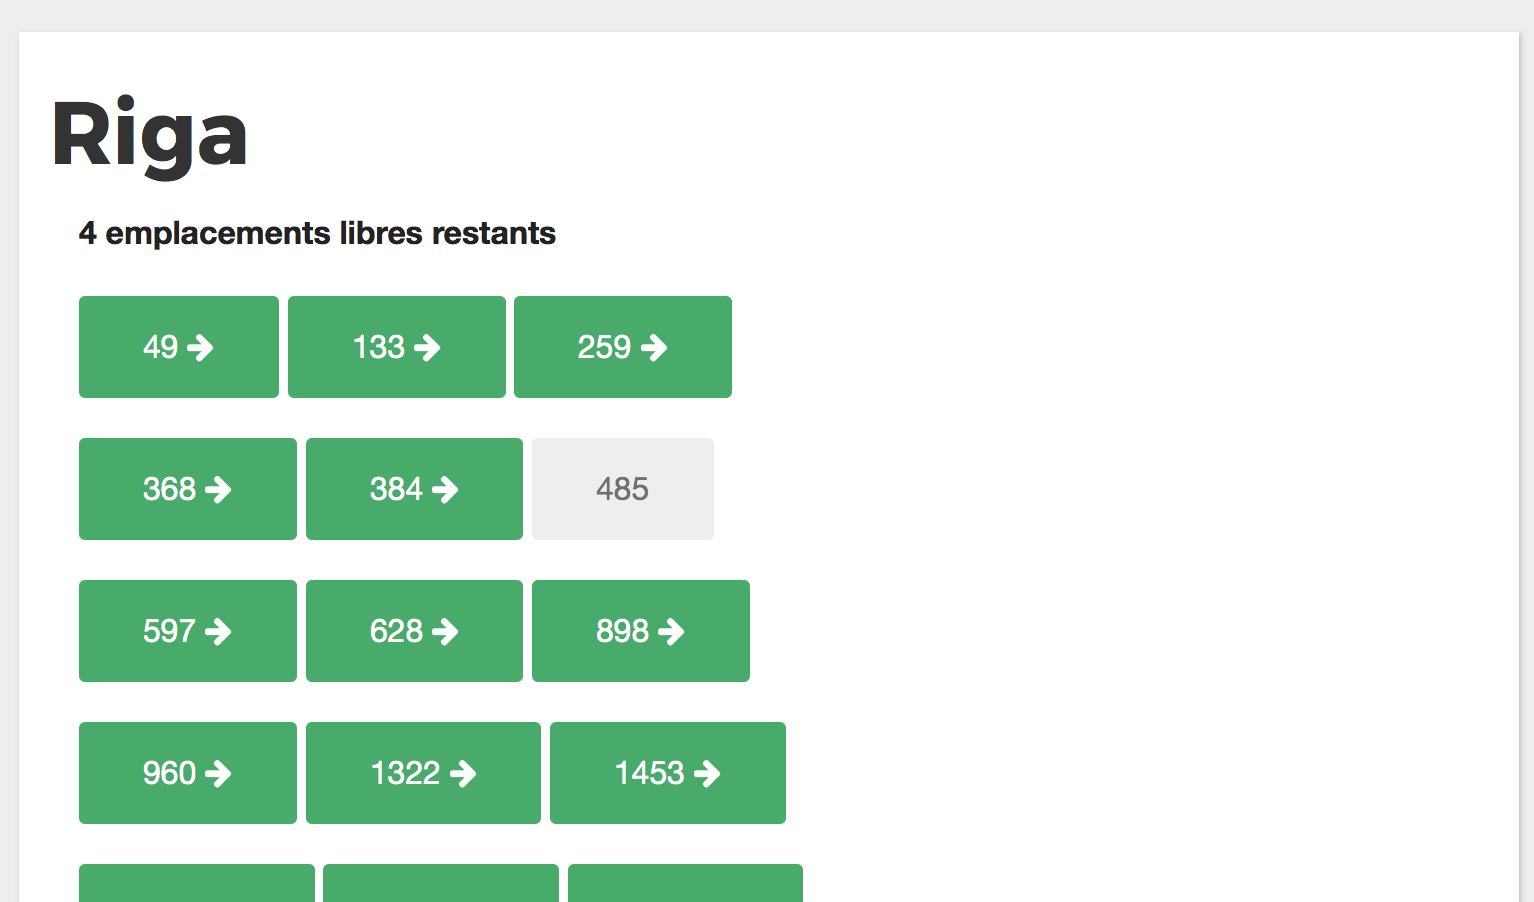
\includegraphics[width=\textwidth]{images/s13.png}
    \caption{Le vélo signalé n'est plus accessible}
    \label{fig-s13}
    \end{figure}
    
    \begin{figure}
    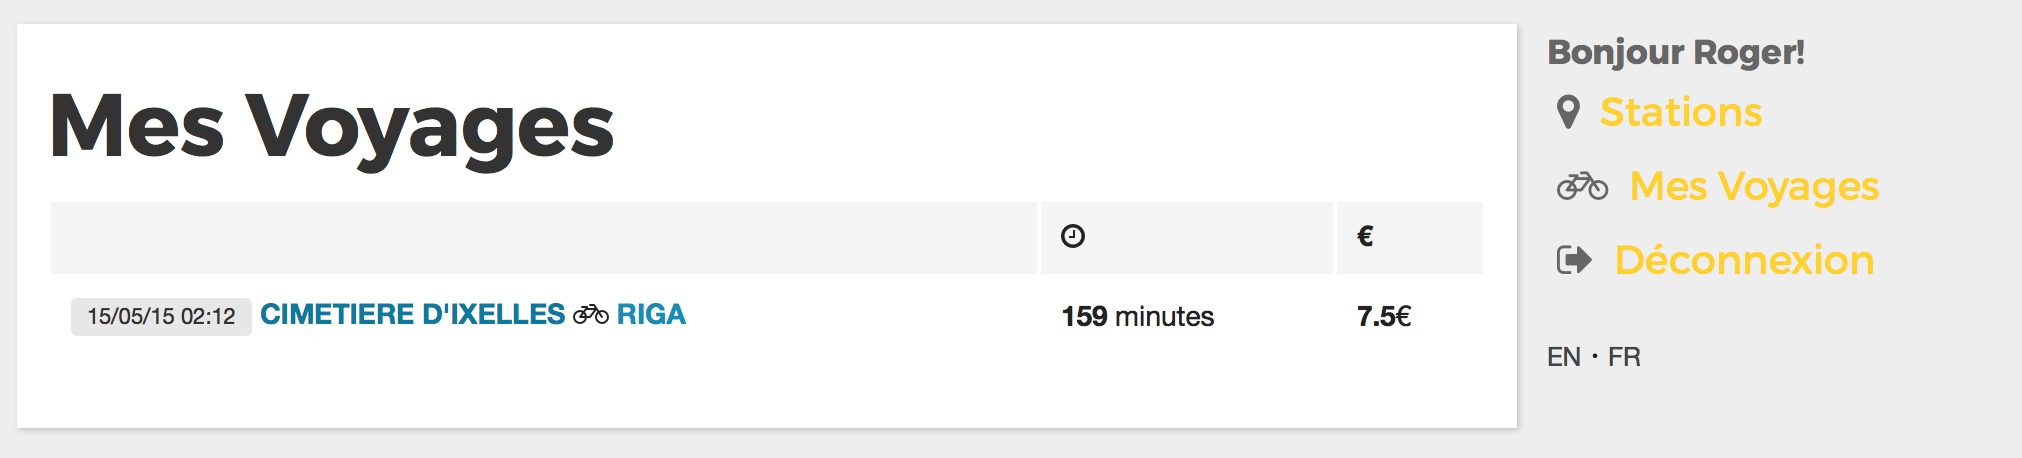
\includegraphics[width=\textwidth]{images/s14.png}
    \caption{Premier trajet effectué}
    \label{fig-s14}
    \end{figure}
    
    \begin{figure}
    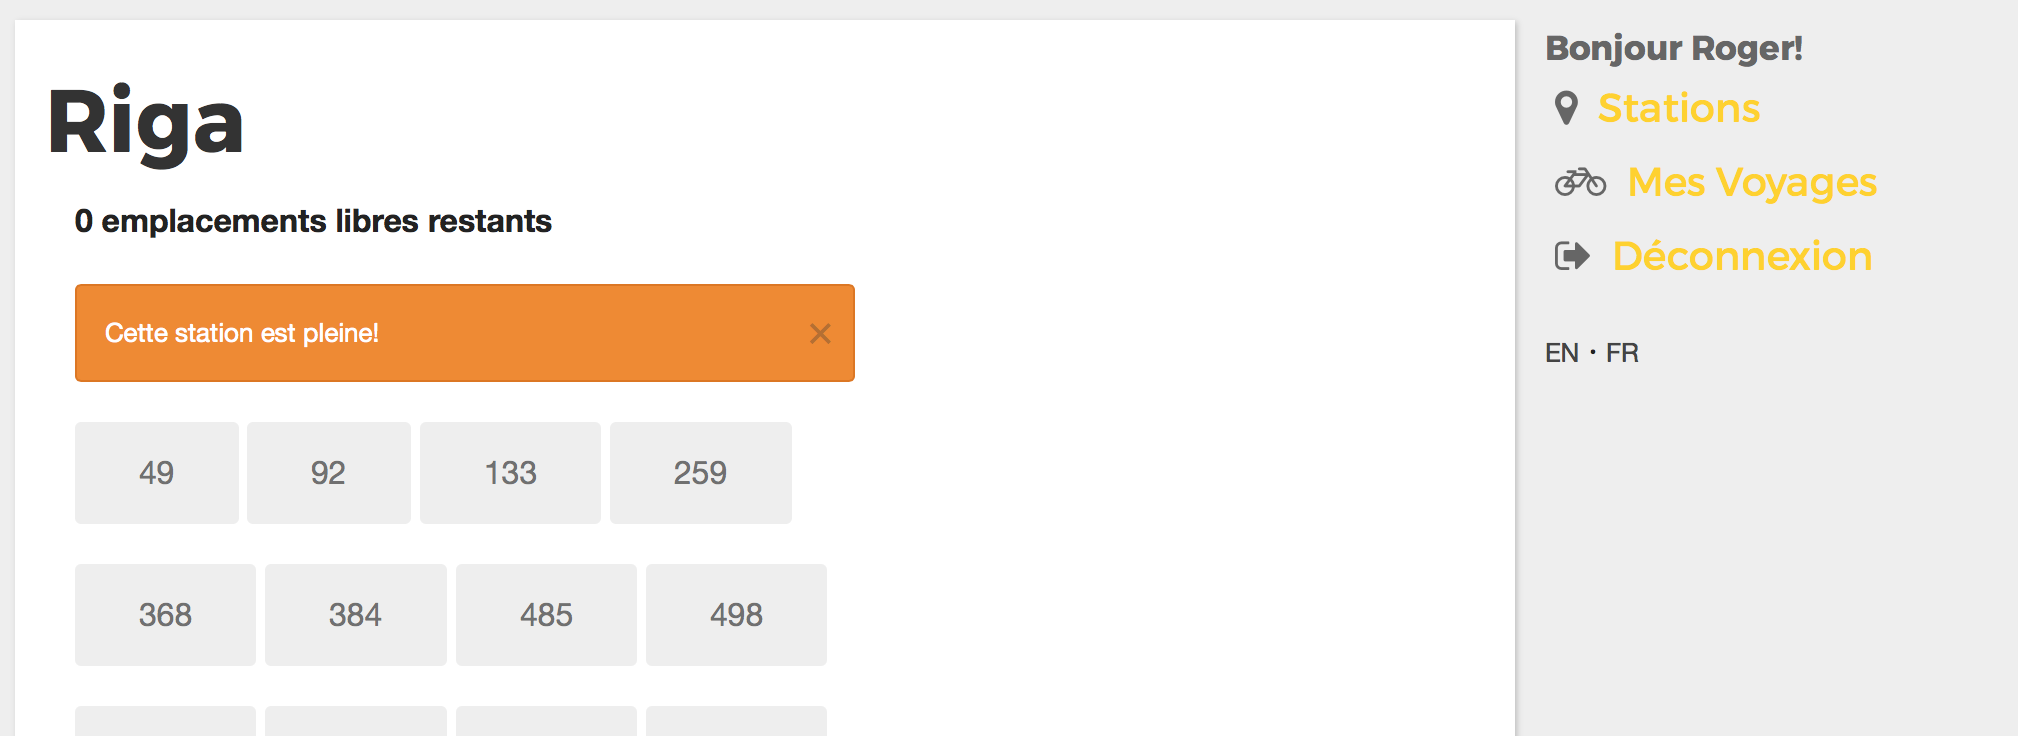
\includegraphics[width=\textwidth]{images/s15.png}
    \caption{Une station pleine}
    \label{fig-s15}
    \end{figure}
    
    \subsection{Apports personnels}
    
    \subsubsection{Achat d'un ticket - utilisateur temporaire}
    On a pu le voir plus haut, quand aucun utilisateur n'est connecté et que la station que l'on regarde dispose d'une borne de paiement, on affiche un formulaire d'achat de ticket (fig \ref{fig-s16}). La procédure est à peu près la même que pour un utilisateur abonné, on va arriver sur une page de bienvenue nous indiquant notre nouveau \texttt{ticketid}(fig \ref{fig-s17}). L'utilisateur a ensuite accès à tous les services Villo!
    
    \begin{figure}
    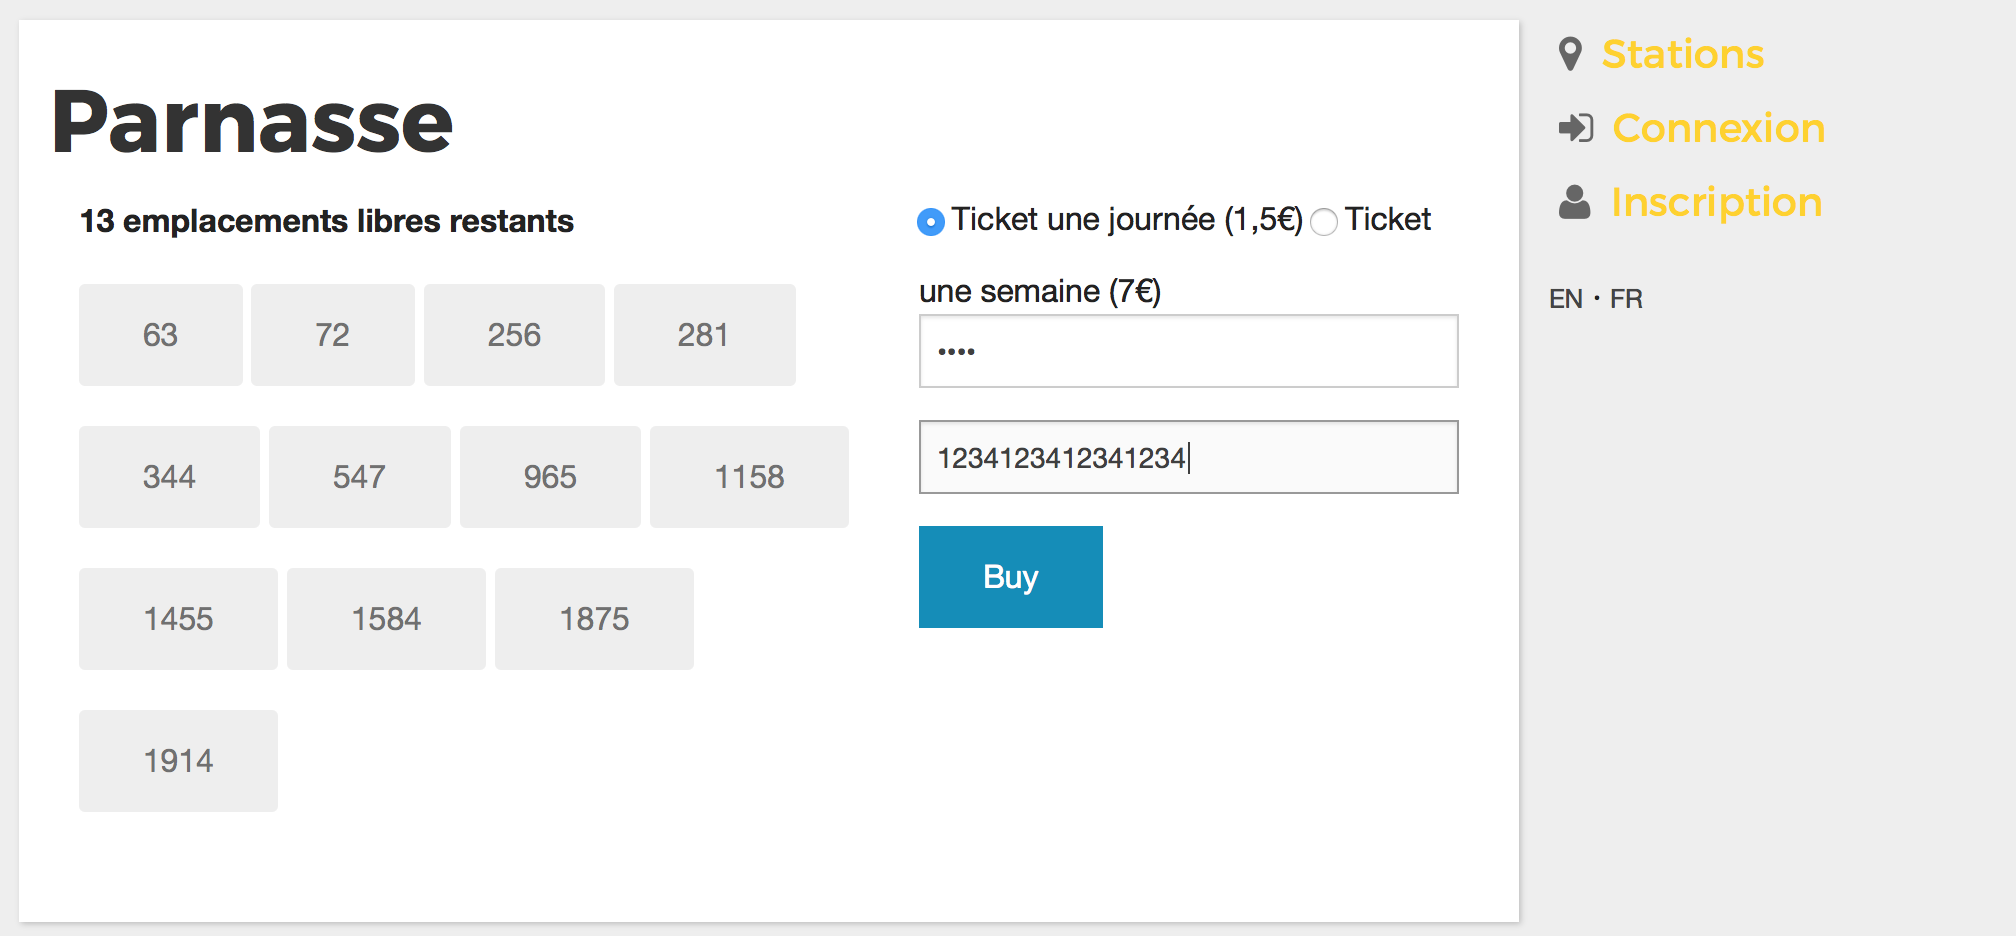
\includegraphics[width=\textwidth]{images/s16.png}
    \caption{Acheter un ticket}
    \label{fig-s16}
    \end{figure}
    
    \begin{figure}
    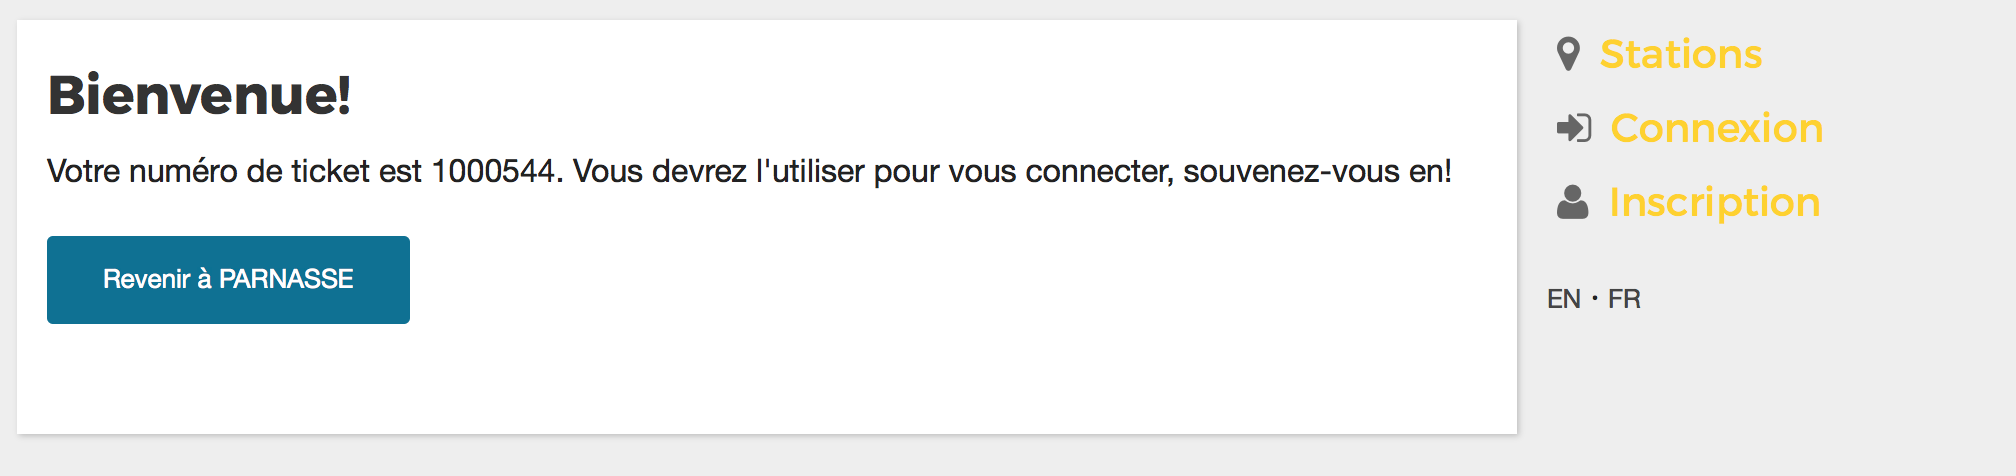
\includegraphics[width=\textwidth]{images/s17.png}
    \caption{Page de bienvenue d'un utilisateur temporaire}
    \label{fig-s17}
    \end{figure}
    
    \subsubsection{Internationalisation}
    Nous avons utilisé Flask-Babel\footnote{https://pythonhosted.org/Flask-Babel/} pour proposer une version du site en anglais et une autre en français. Quelques scripts sont également fournis pour rajouter d'autres expressions à traduire et des instructions claires sont disponibles autant dans le \texttt{README.MD} que sur internet quant à l'ajout de nouveaux langages.\\
    
    Si on clique sur le bouton "EN" du dessous de la colonne de droite, toute l'application se traduit en anglais (fig \ref{fig-s21}). 
    \begin{figure}
    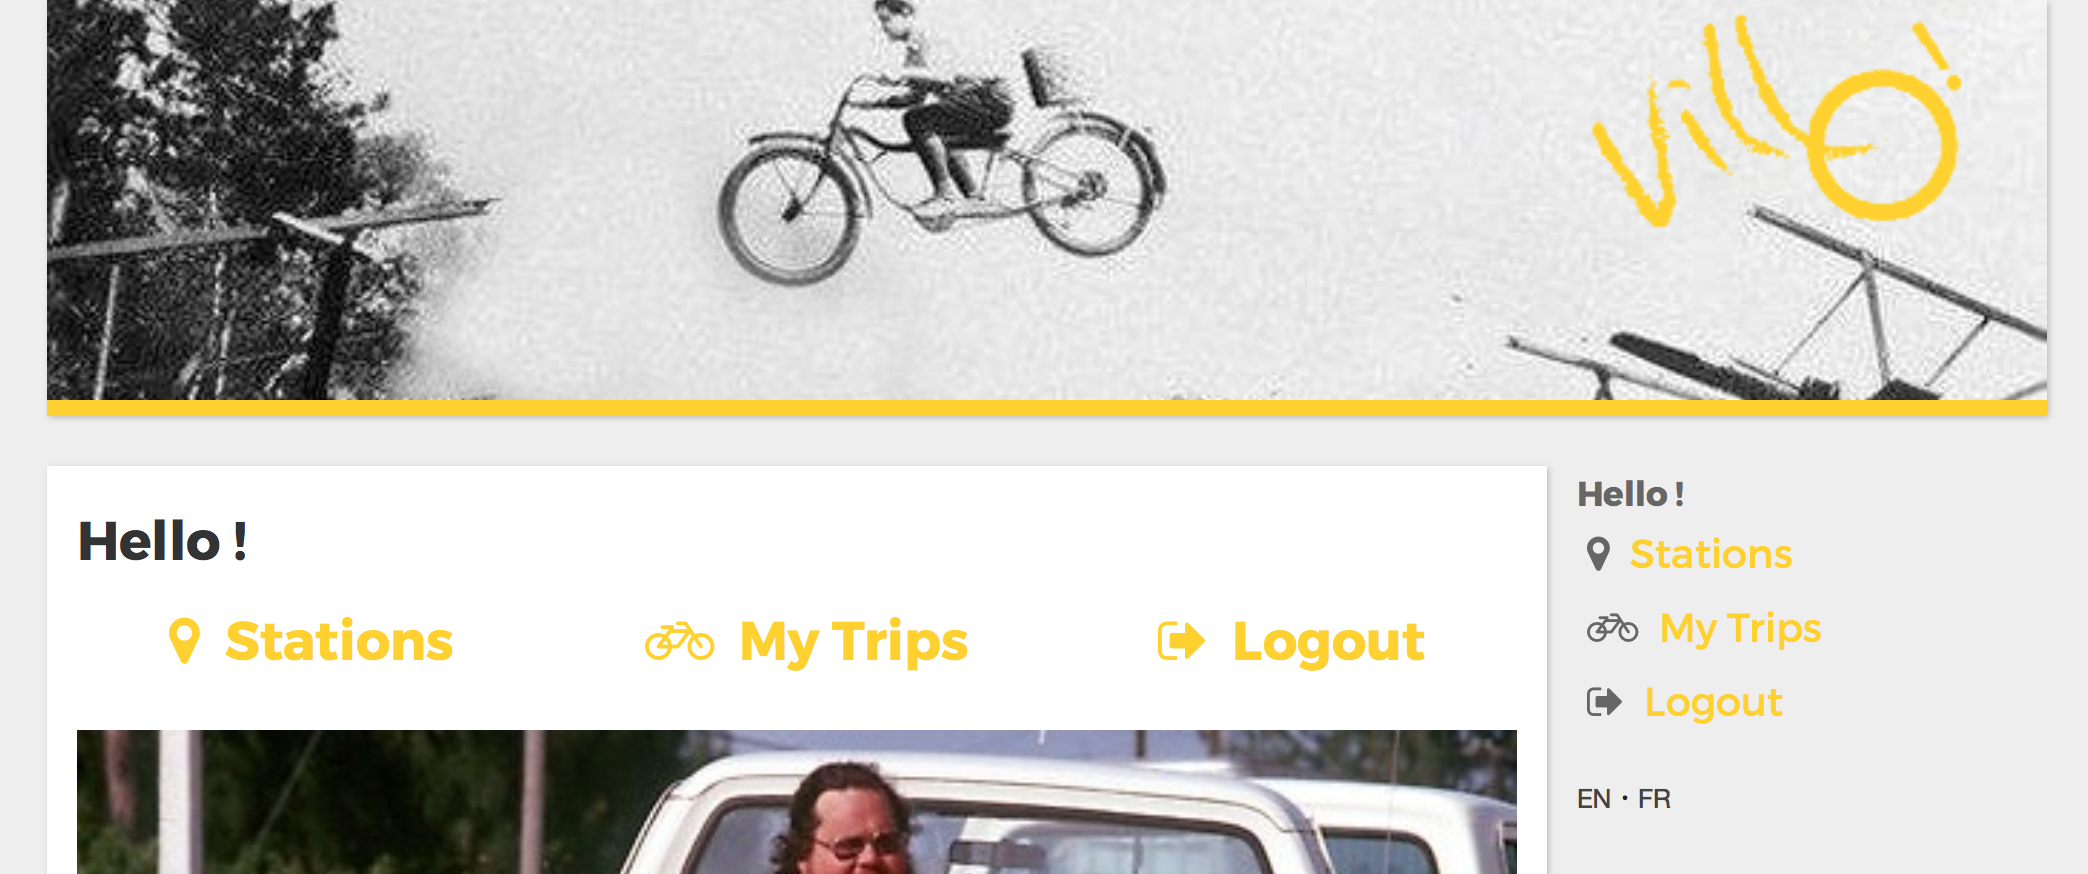
\includegraphics[width=\textwidth]{images/s21.png}
    \caption{L'application en anglais}
    \label{fig-s21}
    \end{figure}
    
    \subsubsection{Google Maps API}
    L'affichage des stations se fait sur une carte Google Maps grâce à l'utilisation de l'API javascript publique. Les limitations de cette API gratuite sont suffisamment amples pour un projet de cette échelle.
    
    \subsubsection{Dashboard administrateur}
    Nous avons décidé de développer un dashboard accessible au chemin \texttt{/admin}, de manière non-sécurisée pour des raisons de clarté et d'accessibilité. On peut y voir la liste des vélos cassés et la station où ils sont rangés, les stations remplies et presque remplies ainsi que les stations vides et presque vides. Ce dashboard peut donc donner une vue d'ensemble intéressante sur les problèmes critiques du système à tout administrateur (fig \ref{fig-s22})
    
    \begin{figure}
    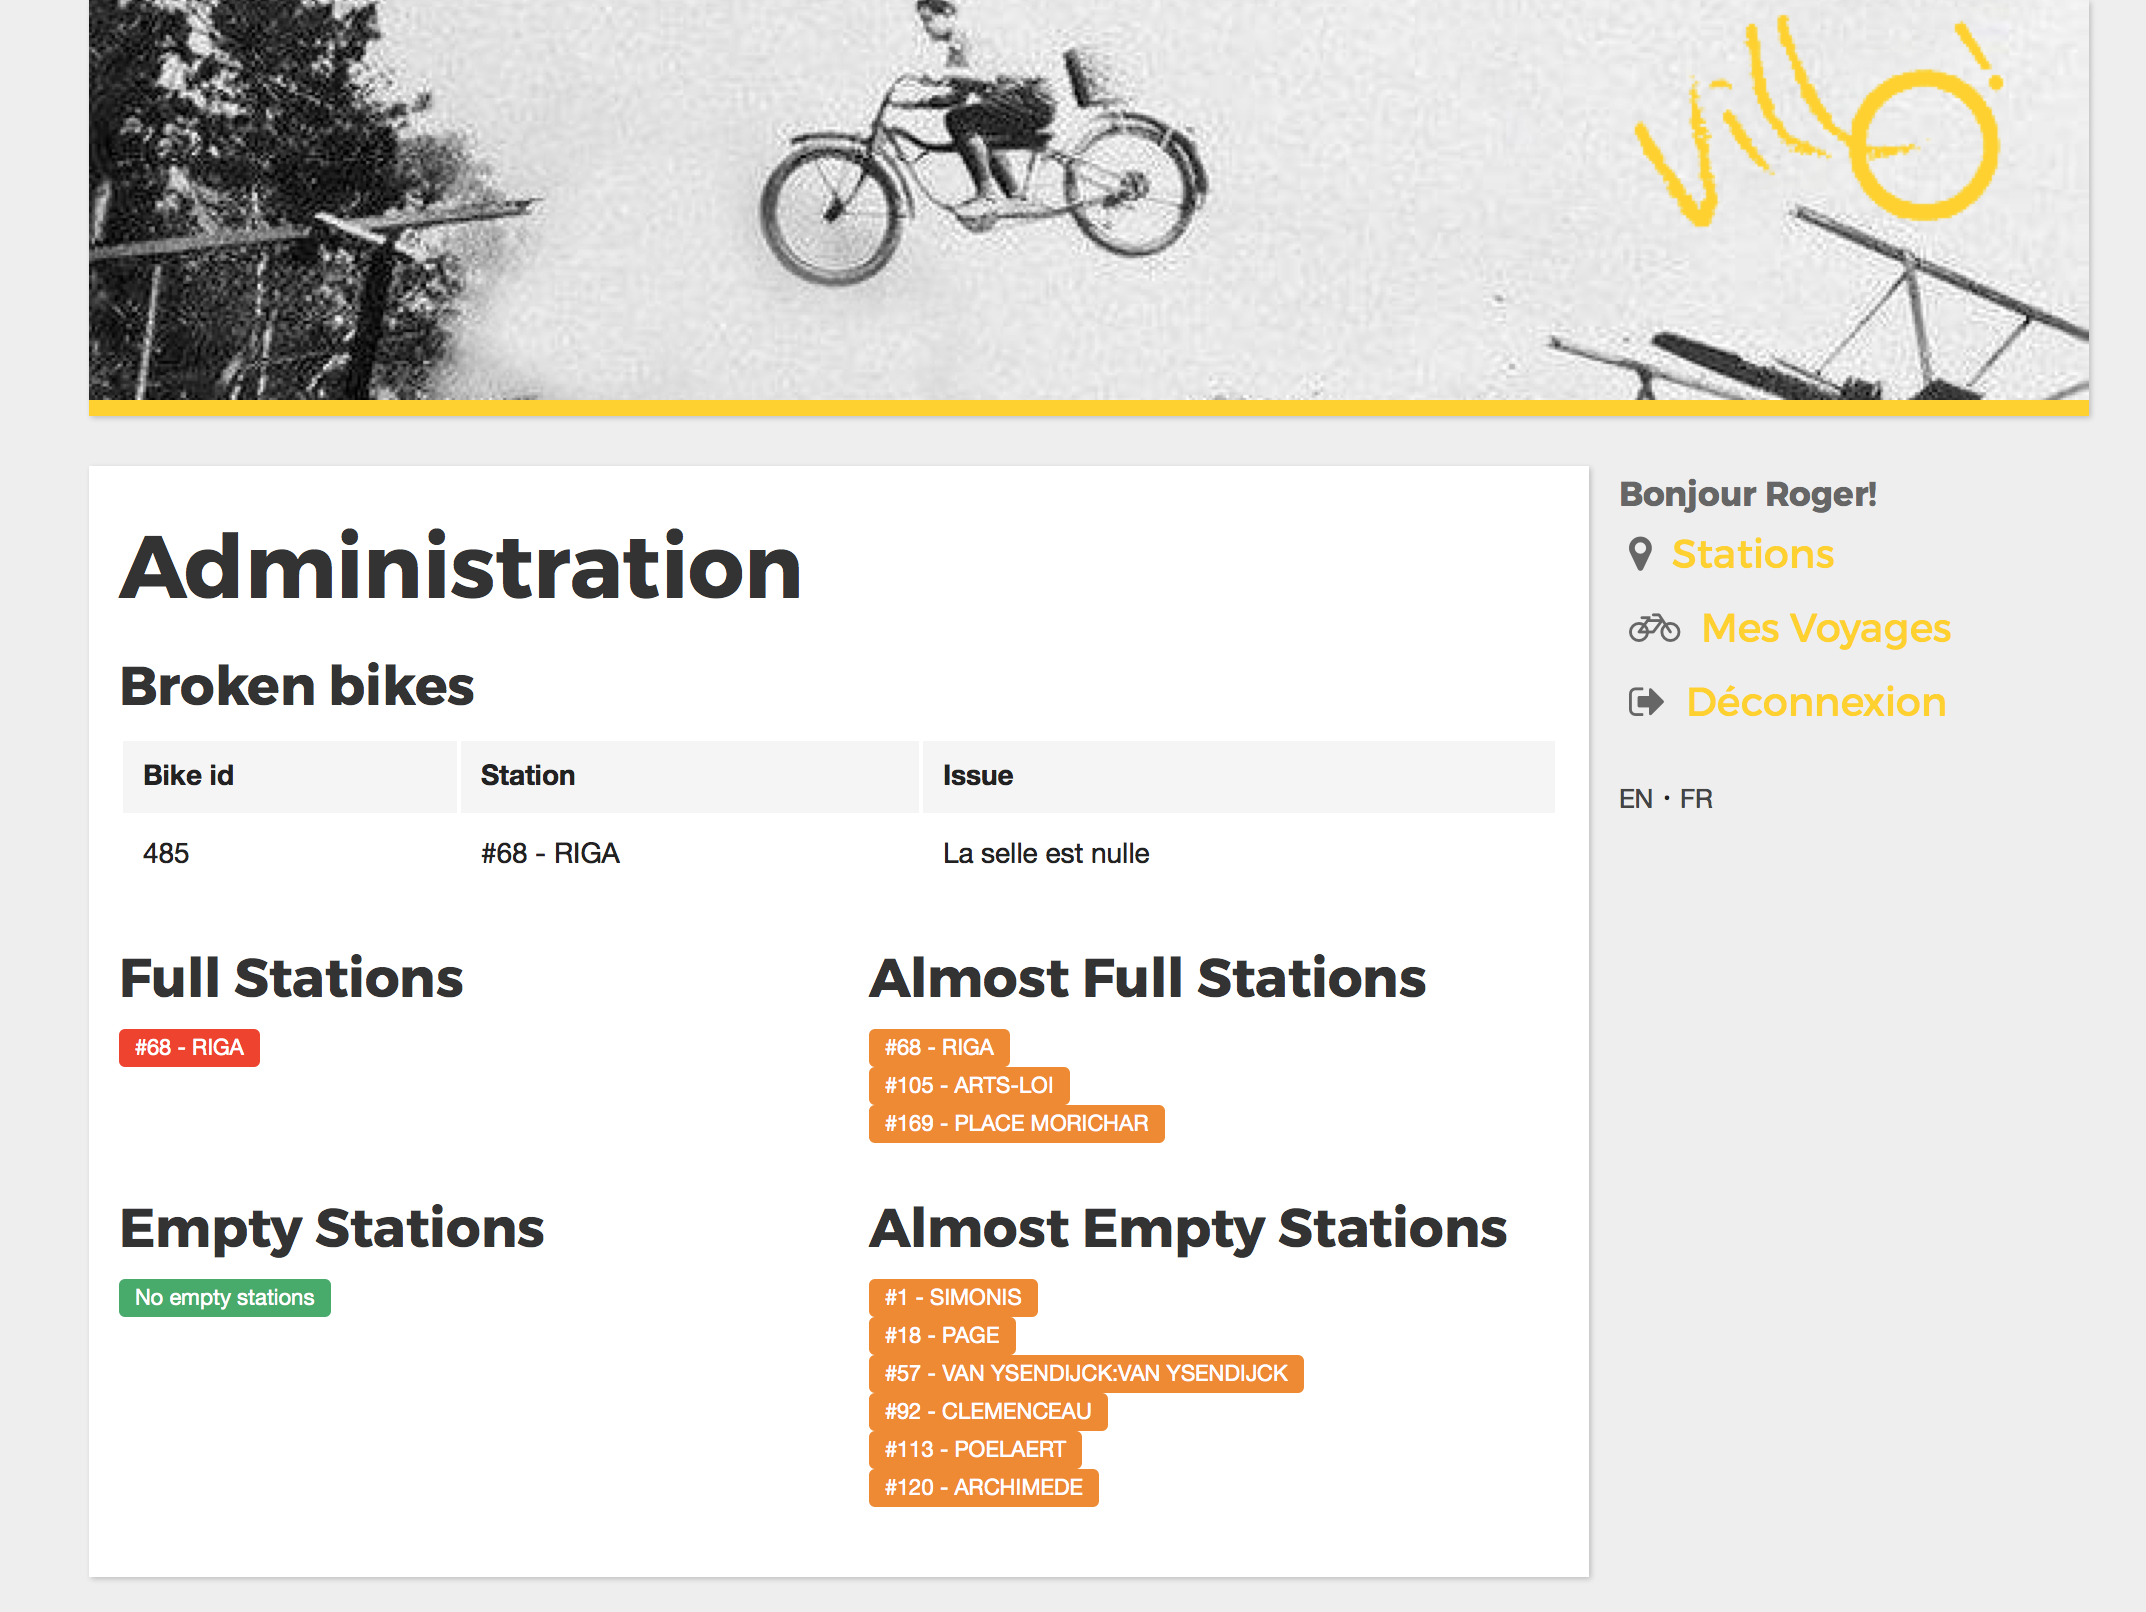
\includegraphics[width=\textwidth]{images/s22.png}
    \caption{Dashboard administrateur}
    \label{fig-s22}
    \end{figure}
    
    \subsubsection{Design}
    Outre le thème jaune imposé par la ville de Bruxelles, nous avons pensé à rendre le site accessible sur des terminaux mobile. Le design est entièrement \textit{responsive} (fig \ref{fig-s23}).
    
    \begin{figure}
    \begin{center}
    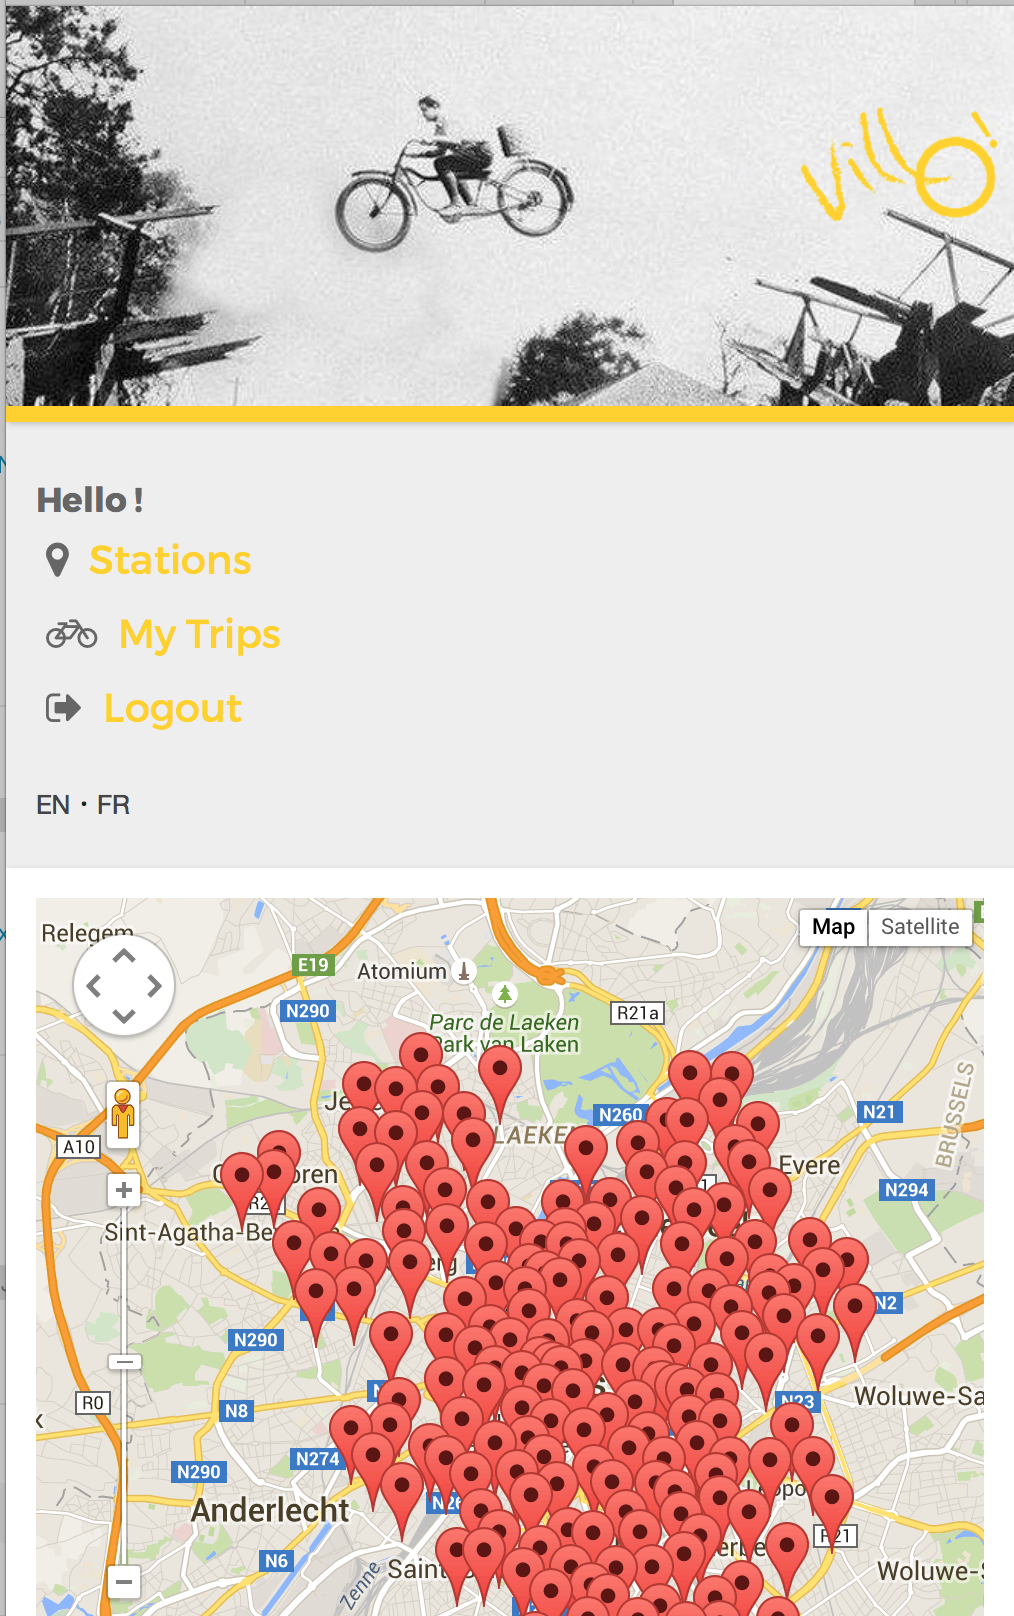
\includegraphics[width=\textwidth/2]{images/s23.png}
    \end{center}
    \caption{Design responsive}
    \label{fig-s23}
    \end{figure}
   
\section{Conclusion}

Ce projet fut très enrichissant, notamment grâce à la diversité des techniques utilisées. Il n'était pas difficile de s'y atteler et de rajouter des fonctionnalités par-ci par-là.\\

En outre, il nous a permis de découvrir plus en profondeur Flask qui est un framework web en Python extrêmement puissant.

\appendix
\section{Extension C pour la distance}
\label{extension-c}
Il est relativement facile de trouver de la documentation sur l'écriture d'extensions pour SQLite3\footnote{https://www.sqlite.org/loadext.html}.

\begin{verbatim}
#include "math.h"
#include <sqlite3ext.h>
#include <stdlib.h> 
SQLITE_EXTENSION_INIT1

static void distance(sqlite3_context *context, int argc, sqlite3_value **argv) {
    double gpsy1 = sqlite3_value_double(argv[0]) * M_PI / 180; // lat in radians
    double gpsx1 = sqlite3_value_double(argv[1]) * M_PI / 180; // long in radians
    double gpsy2 = sqlite3_value_double(argv[2]) * M_PI / 180; // lat in radians
    double gpsx2 = sqlite3_value_double(argv[3]) * M_PI / 180; // long in radians
    double r = 6371.0; // earth's radius in kilometers
    double a, c, distance;

    a = pow(sin((gpsx2-gpsx1)/2),2) + pow(sin((gpsy2-gpsy1)/2), 2) \ 
                    * cos(gpsx1) * cos(gpsx2);
    c = 2 * atan2(sqrt(a), sqrt(1-a));
    distance = r*c;
    sqlite3_result_double(context, distance);
}

#ifdef _WIN32
__declspec(dllexport)
#endif
int sqlite3_distance_init(
  sqlite3 *db, 
  char **pzErrMsg, 
  const sqlite3_api_routines *pApi
){
  int rc = SQLITE_OK;
  SQLITE_EXTENSION_INIT2(pApi);
  sqlite3_create_function_v2(db, "distance", 4, SQLITE_ANY, NULL, distance, \
                    NULL, NULL, NULL);
  return rc;
}
\end{verbatim}



\end{document}